\appendix



\section{Implementation and training details.}\label{sec:implementation}
We carried out experiments using PyTorch~\cite{paszke2017automatic} and a single Nvidia V100 GPU. For all considered backbones (pre-trained on ImageNet), we trained the two last convolutional blocks for one epoch only on the MSLS train set ($\sim$500k pairs), making an efficient use of training data. 
We use the SGD optimizer with initial learning rate of 0.1 for the runs with the GCL function and 0.01 for those with the CL function, and decrease it by a factor of $10^{-1}$ after 250k pairs. For the TB.Places and 7Scene experiments, since they are much smaller datasets we train for 30 epochs, reaching convergence around epoch 15 for both datasets. The initial learning rate is the same as we used for the MSLS experiments, and we decrease it by a factor of $10^{-1}$ after every 5 epochs. All the descriptors are L2-normalized.
%\textbf{ADD DETAILS on TrimBOt and 7Scenes}





%%%%%%%%%%%%%%%%%%%%%%%%%%%%%%%%%%%%%%%%%%%%%%%%%%%%
%%%%%%%%%%%%%%%%%%%%%%%%%%%%%%%%%%%%%%%%%%%%%%%%%%%%
%%%%%%%%%%%%%%%%%%%%%%%%%%%%%%%%%%%%%%%%%%%%%%%%%%%%



\section{Relabeling with image similarity proxies}
\paragraph{2D Field of View Overlap: MSLS data set}




\begin{figure}[!t]
    \centering
\begin{subfigure}{.22\textwidth}
    \includegraphics[width=\textwidth]{figures/4_data/london_query_75_5.jpg}
    \caption{Query}
    \label{fig:msls_london_query}
    \end{subfigure}
~\begin{subfigure}{.22\textwidth}
    \includegraphics[width=\textwidth]{figures/4_data/tokyo_query_50_31.jpg}
    \caption{Query}
    \label{fig:msls_tokyo_query}
    \end{subfigure}
~\begin{subfigure}{.22\textwidth}
    \includegraphics[width=\textwidth]{figures/4_data/sf_query_16_78.jpg}
    \caption{Query}
    \label{fig:msls_sf_query}
    \end{subfigure}
~\begin{subfigure}{.22\textwidth}
    \includegraphics[width=\textwidth]{figures/4_data/trondheim_q_0_0.jpg}
    \caption{Query}
    \label{fig:msls_trondheim_query}
    \end{subfigure}

    
\begin{subfigure}{.22\textwidth}
    \includegraphics[width=\textwidth]{figures/4_data/london_db_75_5.jpg}
    \caption{Positive match}
    \label{fig:msls_london_db}
    \end{subfigure}
~\begin{subfigure}{.22\textwidth}
    \includegraphics[width=\textwidth]{figures/4_data/tokyo_db_50_31.jpg}
    \caption{Positive match}
    \label{fig:msls_tokyo_db}
    \end{subfigure}
~\begin{subfigure}{.22\textwidth}
    \includegraphics[width=\textwidth]{figures/4_data/sf_db_16_78.jpg}
    \caption{Soft negative match}
    \label{fig:msls_sf_db}
    \end{subfigure}
~\begin{subfigure}{.22\textwidth}
    \includegraphics[width=\textwidth]{figures/4_data/trondheim_db_0_0.jpg}
    \caption{Hard negative match}
    \label{fig:msls_trondheim_db}
    \end{subfigure}

    
\begin{subfigure}{.22\textwidth}
    \includegraphics[width=\textwidth]{figures/4_data/london_fov_75_5.png}
    \caption{75.5\% FoV overlap}
    \label{fig:msls_london_fov}
    \end{subfigure}
~\begin{subfigure}{.22\textwidth}
    \includegraphics[width=\textwidth]{figures/4_data/tokyo_fov_50_31.png}
    \caption{50.31\% FoV overlap}
    \label{fig:msls_tokyo_fov}
    \end{subfigure}
~\begin{subfigure}{.22\textwidth}
    \includegraphics[width=\textwidth]{figures/4_data/sf_fov_16_78.png}
    \caption{16.78\% FoV overlap}
    \label{fig:msls_sf_fov}
    \end{subfigure}
~\begin{subfigure}{.22\textwidth}
    \includegraphics[width=\textwidth, trim=1cm 1cm 1cm 1cm, clip]{figures/4_data/trondheim_fov_0.png}
    \caption{0\% FoV overlap}
    \label{fig:msls_trondheim_fov}
    \end{subfigure}

   
    \caption{Example image pairs from the MSLS dataset. The first row shows the query images, the second row shows the corresponding matches from the map set, and the third row shows the estimated 2D FoV overlap. The query image is associated with the red camera, while the map image with the blue camera. The first column shows a positive match with 75.5\% FoV overlap, and many visual features in common. The second column shows a borderline pair: the two images have 50.31\% FoV overlap and some features in common. The third column shows a soft negative match, where the two images have FoV overlap of 16.78\%. The fourth column shows a hard negative match, where the two images are taken by cameras looking in opposite directions, and the FoV overlap is 0\%.}
    \label{fig:msls_fov}
\end{figure}
The authors of MSLS defined a positive match when the retrieved map image falls within 25m and $40^{\circ}$ from the query. We define a similarity measure that satisfies those constraints. Image pairs taken at locations that are closer than 25m and with orientation differences lower than $40^{\circ}$ are expected to have a similarity higher than $50\%$, to be considered similar. Moreover, the borderline cases with distances close to 25m and/or orientation difference near to $40^{\circ}$ should have a similarity close to $50\%$. Hence, we define $r=25m\times2=50m$ and estimate a $\theta$ that gives approximately a $50\%$ FoV overlap for the borderline cases,  i.e. 0m@$40^{\circ}$, and 25m@$0^{\circ}$. For the former, the optimal $\theta$ corresponds to $80^{\circ}$, and for the second latter to $102^{\circ}$. We settle for a value in the middle and define $\theta=90^{\circ}$, which gives $55.63\%$ and $45.01\%$ FoV overlaps in the borderline cases. %, as shown in Fig.~\ref{fig:msls_0m_40deg} and~\ref{fig:msls_25m_0deg}. 
We display  examples of the similarity ground truth for MSLS in Fig.~\ref{fig:msls_fov}. We compute the similarity ground truth for each possible query-map pair, per city. The new annotations are publicly available.

\paragraph{2D Field of View Overlap with IMU and laser tracking: TB-Places dataset}

We present another computation of the 2D field of View overlap to estimate the similarity of image pairs when 6DOF camera pose information is available as metadata next to the images in the dataset. The translation vector $(t_0,t_1)$ and orientation angle $\alpha$ are extracted from the pose vector.

This is the case of the TB-Places dataset~\cite{leyvavallina2019access}, for visual place recognition in gardens, created for the Trimbot2020 project~\cite{strisciuglio2018trimbot2020}. It contains images taken in an experimental garden over three years and includes variations in illumination, season and viewpoint. Each image comes with a 6DOF camera pose, obtained with an IMU and laser tracking, which allows us to estimate a very precise 2D FoV. According to the original paper of the TB-places dataset, we set the FoV angle of the cameras as $\theta = 90^{\circ}$ and the radius as $r=3.5m$. We thus estimate the 2D field of view overlap and use it to re-label the pairs of images contained in the dataset. We provide the similarity ground truth for all possible pairs within W17, the training set. We show some examples of image pairs and their 2D FoV overlap in Fig.~\ref{fig:tbplaces_fov}.


\begin{figure}
  \centering
  \begin{subfigure}{0.3\columnwidth}
\includegraphics[width=\columnwidth]{figures/4_data/W18_positive_q.png}
    \caption{Query}
    \label{fig:tbplaces_positive_query}
  \end{subfigure}
    \begin{subfigure}{0.3\columnwidth}
    \includegraphics[width=\columnwidth]{figures/4_data/W18_positive_db.png}
    \caption{Map}
    \label{fig:tbplaces_positive_db}
  \end{subfigure}
      \begin{subfigure}{0.3\columnwidth}
    \includegraphics[width=\columnwidth, trim=1cm 2cm 1cm 2cm, clip]{figures/4_data/w18_positive_74_21.png}
    \caption{FoV overlap (74\%)}
    \label{fig:tbplaces_positive_fov}
  \end{subfigure}
  \begin{subfigure}{0.3\columnwidth}
  \includegraphics[width=\columnwidth]{figures/4_data/W18_negative_q.png}
      \caption{Query}
    \label{fig:tbplaces_negative_query}
  \end{subfigure}
    \begin{subfigure}{0.3\columnwidth}
\includegraphics[width=\columnwidth]{figures/4_data/W18_negative_db.png}
\caption{Map}
    \label{fig:tbplaces_negative_db}
  \end{subfigure}
  \begin{subfigure}{0.3\columnwidth}
  \includegraphics[width=\columnwidth, trim=1cm 2cm 1cm 2cm, clip]{figures/4_data/w18_negative_40_74.png}
  \caption{FoV overlap (41\%)}
    \label{fig:tbplaces_negative_fov}
  \end{subfigure}
    \caption{Example image pairs from the TB-Places dataset. The first row shows a positive pair with FoV overlap of 74\%. The second row depicts a soft negative pair with FoV overlap equal to 41\%. The red camera corresponds to the query image, while the blue one to the map image.}
    \label{fig:tbplaces_fov}
\end{figure}



\paragraph{3D Surface Overlap: 7Scenes dataset}~\label{sec:3Dfov}


When the 3D reconstruction of a concerned environment is available, we estimate the degree of similarity of image pairs by computing the \emph{3D Surface overlap}. We project a given image with an associated 6DOF camera pose onto the reconstructed pointcloud of the environment. 
We select the subset of 3D points that falls within the boundaries of the image as the image 3D Surface. For an image pair, we compute their 3D Surface overlap as the intersection-over-union (IoU) of the sets of 3D points associated with the two images. \revised{This computation is similar to the \emph{maximum inliers} measure proposed in~\cite{radenovic2018fine}, where it was used as part of a pair-mining strategy that also involved the computation of a distance in the latent space.} We consider, instead, the computed 3D Surface overlap as a proxy for the degree of similarity of a pair of images. 

We use the \emph{3D Surface overlap} to re-annotate the 7Scenes dataset~\cite{Shotton2013}, an indoor localization benchmark, that contains RGBD images taken in seven environments. Each image has an associated 6DOF pose, and a 3D reconstruction of each scene is available. We provide annotations for each possible pair within the training set per scene. %We also compute the test-vs-train similarities for evaluation purposes. }
We show some examples of the 3D Surface overlap in Fig.~\ref{fig:7scenes_fov}. We display the 3D Surface associated to the query image in red, that of the map image in blue and their overlap in magenta. 
%For the binary place recognition classification we consider two images as similar if their 3D FoV Overlap $\psi > 50$\% and dissimilar otherwise.

\begin{figure}

    \centering
    \begin{subfigure}{0.26\columnwidth}
    \includegraphics[width=\columnwidth]{figures/4_data/example_fov_heads_query.png}
    \caption{Query}
    \label{fig:heads_query}
    \end{subfigure}
    \begin{subfigure}{0.26\columnwidth}
    \includegraphics[width=\columnwidth]{figures/4_data/example_fov_heads_map.png}
    \caption{Map}
    \label{fig:heads_db}
    \end{subfigure}
    \begin{subfigure}{0.3\columnwidth}
    \includegraphics[width=\columnwidth,trim=0 0 0 7cm, clip]{figures/4_data/example_fov_heads_noaxis.png}
    \caption{3D Surface overlap (75\%)}
    \label{fig:heads_fov}
    \end{subfigure}
    
    \begin{subfigure}{0.26\columnwidth}
    \includegraphics[width=\columnwidth]{figures/4_data/example_fov_pumpkin_query.png}
    \caption{Query}
    \label{fig:pumpkin_query} 
    \end{subfigure}
    \begin{subfigure}{0.26\columnwidth}
\includegraphics[width=\columnwidth]{figures/4_data/example_fov_pumpkin_map.png}
    \caption{Map}
    \label{fig:pumpkin_db}\end{subfigure}
    \begin{subfigure}{0.32\columnwidth}
    \includegraphics[width=\columnwidth]{figures/4_data/example_fov_pumpkin_noaxis.png}
    \caption{3D Surface overlap (50\%)}
    \label{fig:pumpkin_fov}
    \end{subfigure}
    
    \begin{subfigure}{0.26\columnwidth}
    \includegraphics[width=\columnwidth]{figures/4_data/example_fov_fire_query.png}
   \caption{Query}
    \label{fig:fire_query} 
    \end{subfigure}
    \begin{subfigure}{0.26\columnwidth}
    \includegraphics[width=\columnwidth]{figures/4_data/example_fov_fire_map.png}
   \caption{Map}
    \label{fig:fire_db} 
    \end{subfigure}
    \begin{subfigure}{0.3\columnwidth}
    \includegraphics[width=\columnwidth]{figures/4_data/example_fov_fire_noaxis.png}
    \caption{3D Surface overlap (25\%)}
    \label{fig:fire_fov}
    \end{subfigure}
    \caption{3D Surface overlap examples from the 7Scenes dataset. The first row shows a positive pair with 3D Surface overlap of 75\%. The second row depicts a borderline pair with 50\% 3D Surface overlap. The last row shows a soft negative image pair with 25\% 3D Surface overlap.
    The red pointcloud corresponds to the query 3D Surface, the blue one is the map, and the magenta represents the overlap between them.}
    \label{fig:7scenes_fov}
\end{figure}


\subsection{Field of View vs. Distance}

We studied the relation among translation distance, rotation difference and the resulting FoV overlap measure. 
For that, we selected a subset of pairs of the MSLS training set and measured how the value of the FoV overlap varies with respect to the position and orientation difference of the image pairs. 
In Fig.~\ref{fig:supp_fov_tr}, we plot the relationship between the  translation distance and the value of the FoV overlap. We observed a somewhat linear relationship between increasing translation distance and decreasing FoV overlap. Moreover, many image pairs with FoV overlap of approximately 50\% were taken at a distance of about 25m. The variance observed in Fig.~\ref{fig:supp_fov_tr} is attributable to the orientation changes. Indeed, the relation between FoV overlap and orientation difference is less clear (see Fig.~\ref{fig:supp_fov_rot}). However, the pairs with smaller orientation distance tend to have a generally higher FoV overlap. 
We plot the relation of the FoV overlap with both translation and orientation distance in a 3-dimensional plane in Fig.~\ref{fig:supp_fov_3d}, and as a heatmap in Fig.~\ref{fig:supp_fov_colormap}. 
Rotation and translation distance jointly influence the FoV overlap: the smaller the translation and orientation distance, the higher the similarity. Furthermore, the higher one of the distance measures, the lower the computed FoV overlap, and thus the annotated ground truth similarity.

\begin{figure}[!t]
    \begin{subfigure}{.45\columnwidth}
    \centering
    \hspace{-15mm}\includegraphics[width=\columnwidth]{figures/appendix/fov/fov_tr.pdf}
    \caption{}
    \label{fig:supp_fov_tr}
    \end{subfigure}
    ~\begin{subfigure}{.45\columnwidth}
\centering
    \includegraphics[width=\columnwidth]{figures/appendix/fov/fov_rot.pdf}
    \caption{}
        \label{fig:supp_fov_rot}
        \end{subfigure}\\
         \begin{subfigure}{.45\columnwidth}
\centering
    \includegraphics[width=\columnwidth]{figures/appendix/fov/fov_3d.pdf}
    \caption{}
        \label{fig:supp_fov_3d}
        \end{subfigure}~         \begin{subfigure}{.45\columnwidth}
\centering
    \includegraphics[width=\columnwidth]{figures/appendix/fov/fov_colormap.pdf}
    \caption{}
    \label{fig:supp_fov_colormap}
    \end{subfigure}
    \caption{Relation of 2D FoV overlap with translation and orientation distance (computed using a subset of MSLS validation set).} % This data is computed from a subset of the MSLS training set.}
    \label{fig:supp_fov}
\end{figure}



%%%%%%%%%%%%%%%%%%%%%%%%%%%%%%%%%%%%%%%%%%%%%%%%%%%%
%%%%%%%%%%%%%%%%%%%%%%%%%%%%%%%%%%%%%%%%%%%%%%%%%%%%
%%%%%%%%%%%%%%%%%%%%%%%%%%%%%%%%%%%%%%%%%%%%%%%%%%%%

\section{CL vs GCL: comparison of  latent space }

In Fig.~\ref{fig:tsne}, we show the 2D projection of the difference of the latent space representations of 2000 image pairs (1000 positive and 1000 negative) randomly selected from the Copenhagen set of the MSLS validation set. For each pair, we compute the difference between the map and the query image descriptors. We use this as input to t-SNE~\cite{tsne}, which projects the descriptors onto a 2D space. We visualize the vectors produced by two models with a ResNet50-GeM backbone, one trained using the CL function (Fig.~\ref{fig:tsneCL}) and the other using the GCL (Fig.~\ref{fig:tsneGCL}) function. The effect of the proposed GCL function is evident in the better regularized latent space, where the representation of similar image pairs (blue dots) are more consistently distributed towards the center of the space. The representations learned using the CL function, instead, form a more scattered and noisy distribution.






%%%%%%%%%%%%%%%%%%%%%%%%%%%%%%%%%%%%%%%%%%%%%%%%%%%%
%%%%%%%%%%%%%%%%%%%%%%%%%%%%%%%%%%%%%%%%%%%%%%%%%%%%
%%%%%%%%%%%%%%%%%%%%%%%%%%%%%%%%%%%%%%%%%%%%%%%%%%%%
\section{Large-scale VPR: additional results}


\begin{figure}[!t]
  \centering
  \begin{subfigure}{0.48\columnwidth}
  \includegraphics[width=\columnwidth]{figures/appendix/tsne/resnet50-GeM-CL-nowhitening-tsne-cph.jpg}
  \caption{ResNet50-GeM-CL}
    \label{fig:tsneCL}
  \end{subfigure}
  \hfill
  \begin{subfigure}{0.48\columnwidth}
\includegraphics[width=\columnwidth]{figures/appendix/tsne/resnet50-GeM-GCL-nowhitening-tsne-cph.jpg}
\caption{ResNet50-GeM-GCL}
\label{fig:tsneGCL}
  \end{subfigure}
    \caption{Visualization of the learned latent space. We selected 1000 random positive pairs and 1000 random negative pairs from the MSLS Copenhagen set, computed the differences between their representations and projected them into a 2D space using t-SNE.}
    \label{fig:tsne}
\end{figure}






\begin{table}[t!]
\centering
\caption{Detailed results on the Extended CMU dataset. The $^\star$ denotes the models for which PCA whitening has been applied. }
\label{tab:cmu_detailed}
\resizebox{\columnwidth}{!}{%
\setlength\tabcolsep{1.5pt}
\begin{tabular}{@{}lcccc@{}}
\toprule
\textbf{} & \textbf{Mean} & \textbf{Urban} & \textbf{Suburban} & \textbf{Park} \\ 
\textbf{Method} & \textbf{\begin{tabular}[c]{@{}c@{}}0.25/0.5/10m \\ 2/5/10$\degree$\end{tabular}} & \textbf{\begin{tabular}[c]{@{}c@{}}0.25/0.5/10m \\ 2/5/10$\degree$\end{tabular}} & \textbf{\begin{tabular}[c]{@{}c@{}}0.25/0.5/10m \\ 2/5/10$\degree$\end{tabular}} & \textbf{\begin{tabular}[c]{@{}c@{}}0.25/0.5/10m \\ 2/5/10$\degree$\end{tabular}} \\\midrule
%NetVLAD-64-Pitts30k & 5.3 / 15.9 / 66.3 & 10.7 / 27.8 / 84.1 & 2.9 / 11.2 / 63.5 & 2.4 / 8.9 / 50.1 \\
%NetVLAD-64-Pitts30k$^\star$ & 5.8 / 17.6 / 70.3 & 11.6 / 30.3 / 87.5 & 3.3 / 12.5 / 68 & 2.7 / 10.2 / 54.2 \\
NetVLAD-64 & 1.3 / 4.5 / 31.9 & 2.9 / 8.4 / 49.6 & 0.8 / 3.4 / 29.7 & 0.3 / 1.6 / 15.2 \\
NetVLAD-64$^\star$ & 3.9 / 12.1 / 58.4 & 7.6 / 20.3 / 77.2 & 2.6 / 9.7 / 58.9 & 1.6 / 6.3 / 37.0 \\
NetVLAD-16 & 1.7 / 5.5 / 39.1 & 3.7 / 10.0 / 57.3 & 1.1 / 4.5 / 38.6 & 0.4 / 1.9 / 19.8 \\
NetVLAD-16$^\star$ & 4.4 / 13.7 / 61.4 & 8.4 / 22.1 / 76.9 & 3.0 / 11.4 / 63.1 & 1.9 / 7.4 / 41.9 \\
% AP-GeM$^\star$ & 4.9 / 14.7 / 65.2 & 9.8 / 25.2 / 82.6 & 2.8 / 10.9 / 65.3 & 2.1 / 8 / 45.9 \\
% NetVLAD-SARE$^\star$ & \textbf{6.4} / \textbf{19.4} / \textbf{75.5} & \textbf{12.5} / \textbf{32.4 }/ \textbf{90.7} & \textbf{3.9} / \textbf{14.7 }/ \textbf{76.3} & 3.0 / 11.3 / 57.6 \\
\midrule
VGG-avg-CL & 0.9 / 3.0 / 22.7 & 2.0 / 5.8 / 39.4 & 0.6 / 2.3 / 21 & 0.2 / 0.7 / 6.5 \\
VGG-avg-GCL & 2.3 / 7.2 / 43.3 & 4.7 / 13.0 / 64.3 & 1.6 / 5.8 / 43.4 & 0.7 / 2.5 / 19.8 \\
VGG-avg-CL$^\star$ & 2.1 / 6.6 / 34.9 & 4.4 / 12.3 / 54.1 & 1.1 / 4.4 / 30.5 & 0.9 / 3.1 / 19.4 \\
VGG-avg-GCL$^\star$ & 3.7 / 11.2 / 52.5 & 7.2 / 19.1 / 70.8 & 2.1 / 8.2 / 50.4 & 1.8 / 6.2 / 35.1 \\
VGG-GeM-CL & 2.8 / 8.6 / 44.5 & 5.7 / 15.2 / 63.7 & 1.6 / 6.4 / 44.9 & 1.1 / 4.2 / 22.8 \\
VGG-GeM-GCL & 3.6 / 11.2 / 55.8 & 6.8 / 18.5 / 73.6 & 2.5 / 9.2 / 57.3 & 1.5 / 5.6 / 34.2 \\
VGG-GeM-CL$^\star$ & 4.4 / 13.4 / 56.5 & 8.4 / 21.5 / 72.1 & 2.6 / 10 / 55.2 & 2.3 / 8.7 / 40.8 \\
VGG-GeM-GCL$^\star$ & 5.7 / 17.1 / 66.3 & 10.4 / 26.8 / 82.2 & 3.8 / 13.8 / 67.8 & 2.8 / 10.7 / 46.7 \\\midrule
ResNet50-avg-CL & 2.6 / 7.8 / 43.4 & 5.6 / 14.9 / 64.6 & 1.4 / 5.5 / 42.6 & 0.8 / 2.9 / 21.1 \\
ResNet50-avg-GCL & 3.1 / 9.7 / 55.1 & 6 / 16.7 / 73.6 & 2.0 / 7.7 / 56.8 & 1.2 / 4.7 / 32.5 \\
ResNet50-avg-CL$^\star$ & 4.7 / 13.8 / 50.8 & 9.5 / 24.1 / 70.5 & 2.7 / 9.7 / 48.8 & 2.1 / 7.6 / 31.7 \\
ResNet50-avg-GCL$^\star$ & 5.4 / 16.2 / 66.5 & 10.2 / 26.5 / 81.8 & 3.5 / 12.5 / 69.8 & 2.6 / 9.6 / 45.3 \\
ResNet50-GeM-CL & 3.2 / 9.6 / 49.5 & 6.5 / 17.3 / 70.7 & 1.9 / 7.0 / 49.3 & 1.2 / 4.3 / 26.3 \\
ResNet50-GeM-GCL & 3.8 / 11.8 / 61.6 & 7.4 / 19.9 / 79.2 & 2.4 / 9.4 / 64.8 & 1.5 / 6.1 / 38.1 \\
ResNet50-GeM-CL$^\star$ & 4.7 / 13.4 / 51.6 & 9.5 / 23.9 / 73.5 & 2.8 / 9.6 / 49.7 & 1.9 / 6.8 / 30.0 \\
ResNet50-GeM-GCL$^\star$ & 5.4 / 16.5 / 69.9 & 10.1 / 26.3 / 84.5 & 3.5 / 13.4 / 74.1 & 2.6 / 9.8 / 48.2 \\\midrule
ResNet152-avg-CL & 3.0 / 9.2 / 49.9 & 6.2 / 16.4 / 70.4 & 1.9 / 6.9 / 48.7 & 1.0 / 4.1 / 28.9 \\
ResNet152-avg-GCL & 3.6 / 11.0 / 61.2 & 7.0 / 18.9 / 78.8 & 2.3 / 8.4 / 62.6 & 1.4 / 5.5 / 39.9 \\
ResNet152-avg-CL$^\star$ & 4.8 / 14.3 / 59.9 & 9.4 / 24 / 77.3 & 3.0 / 10.9 / 61 & 2 / 8 / 39.3 \\
ResNet152-avg-GCL$^\star$ & 5.7 / 17.0 / 66.5 & 10.8 / 27.3 / 82.0 & 3.7 / 13.5 / 68.9 & 2.6 / 10.1 / 46.3 \\
ResNet152-GeM-CL & 3.2 / 9.7 / 52.2 & 6.7 / 17.7 / 73.9 & 2.1 / 7.3 / 52.8 & 0.9 / 4.1 / 27.6 \\
ResNet152-GeM-GCL & 3.6 / 11.3 / 63.1 & 6.9 / 18.8 / 79.3 & 2.5 / 9.0 / 64.3 & 1.3 / 6.0 / 43.6 \\
ResNet152-GeM-CL$^\star$ & 4.8 / 14.2 / 55.0 & 9.6 / 24.5 / 75.2 & 3.0 / 10.5 / 54.3 & 1.9 / 7.5 / 33.6 \\
ResNet152-GeM-GCL$^\star$ & 5.3 / 16.1 / 66.4 & 9.9 / 25.8 / 81.6 & 3.5 / 12.8 / 69.3 & 2.4 / 9.7 / 46 \\\midrule
ResNext-avg-CL & 2.0 / 6.1 / 40.0 & 4.6 / 12.2 / 63.6 & 1.2 / 4.4 / 38.5 & 0.3 / 1.7 / 16.0 \\
ResNext-avg-GCL & 3.3 / 10.2 / 57.7 & 6.7 / 17.9 / 77.8 & 2.1 / 8.1 / 58.1 & 1.2 / 4.4 / 35.0 \\
ResNext-avg-CL$^\star$ & 4.6 / 13.4 / 58.6 & 9.3 / 23.2 / 78 & 2.8 / 10.1 / 59 & 1.7 / 6.7 / 36.5 \\
ResNext-avg-GCL$^\star$ & 5.6 / 16.6 / 70.7 & 10.4 / 26.6 / 85.1 & 3.7 / 13.4 / 73.2 & 2.6 / 9.8 / 51.6 \\
ResNext-GeM-CL & 2.9 / 9.0 / 52.6 & 5.9 / 15.6 / 70.2 & 1.7 / 6.8 / 53.0 & 1.2 / 4.7 / 32.6 \\
ResNext-GeM-GCL & 3.5 / 10.5 / 58.8 & 6.5 / 17.7 / 77.8 & 2.5 / 8.7 / 59.7 & 1.3 / 5.0 / 36.6 \\
ResNext-GeM-CL$^\star$ & 4.9 / 14.4 / 61.7 & 9.4 / 24 / 80.2 & 3.1 / 11.1 / 63.8 & 2.2 / 8.0 / 38.6 \\
ResNext-GeM-GCL$^\star$ & 6.1 / 18.2 / 74.9 & 11.1 / 28.7 / 87.4 & 4.2 / 14.6 / 77.4 & \textbf{3.1} / \textbf{11.1} / \textbf{57.7 }\\ \bottomrule
\end{tabular}
}
\end{table}

\subsection{RobotCar Seasons v2 and Ext. CMU Seasons}

We provide results divided by type of environment for the Extended CMU dataset in Table~\ref{tab:cmu_detailed}. We observed that all models (ours and SoTA) tend to reach a higher performance on the urban images. This is logical, as they are all trained on the MSLS dataset with images of mainly urban areas. 

We also provide detailed results for the RobotCar Seasons v2 dataset, organized by weather and illumination conditions, in Table~\ref{tab:robotcar_extended}. We observe that all methods obtain a higher successful localization rate on day conditions, and the GCL-based methods (especially with a ResNet backbone) tend to have goof performance on the night-time subsets as well. The MSLS train dataset includes images taken at night, although underrepresented, so it is interesting that GCL based models can localize images under these conditions.

\begin{table*}[!t]
\centering
\caption{Detailed results on the RobotCar Seasons v2 dataset, divided by wheather and ilumination conditions. The symbol $^\star$ denotes the models for which PCA whitening has been applied.}
\label{tab:robotcar_extended}
\renewcommand{\arraystretch}{0.95}
\resizebox{\textwidth}{!}{%
\setlength\tabcolsep{1.75pt}
\begin{tabular}{@{}l|c|c|c|c|c|c|c|c|c|c|c|c@{}}
\toprule
\textbf{} & \textbf{night rain} & \textbf{night} & \textbf{night all} & \textbf{overcast winter} & \textbf{sun} & \textbf{rain} & \textbf{snow} & \textbf{dawn} & \textbf{dusk} & \textbf{overcast summer} & \textbf{day all} & \textbf{mean} \\
\textbf{Method} & \textbf{\begin{tabular}[c]{@{}c@{}}0.25/0.5/10m \\ 2/5/10$\degree$\end{tabular}} & \textbf{\begin{tabular}[c]{@{}c@{}}0.25/0.5/10m \\ 2/5/10$\degree$\end{tabular}} & \textbf{\begin{tabular}[c]{@{}c@{}}0.25/0.5/10m \\ 2/5/10$\degree$\end{tabular}} & \textbf{\begin{tabular}[c]{@{}c@{}}0.25/0.5/10m \\ 2/5/10$\degree$\end{tabular}} & \textbf{\begin{tabular}[c]{@{}c@{}}0.25/0.5/10m \\ 2/5/10$\degree$\end{tabular}} & \textbf{\begin{tabular}[c]{@{}c@{}}0.25/0.5/10m \\ 2/5/10$\degree$\end{tabular}} & \textbf{\begin{tabular}[c]{@{}c@{}}0.25/0.5/10m \\ 2/5/10$\degree$\end{tabular}} & \textbf{\begin{tabular}[c]{@{}c@{}}0.25/0.5/10m \\ 2/5/10$\degree$\end{tabular}} & \textbf{\begin{tabular}[c]{@{}c@{}}0.25/0.5/10m \\ 2/5/10$\degree$\end{tabular}} & \textbf{\begin{tabular}[c]{@{}c@{}}0.25/0.5/10m \\ 2/5/10$\degree$\end{tabular}} & \textbf{\begin{tabular}[c]{@{}c@{}}0.25/0.5/10m \\ 2/5/10$\degree$\end{tabular}} & \textbf{\begin{tabular}[c]{@{}c@{}}0.25/0.5/10m \\ 2/5/10$\degree$\end{tabular}} \\ \midrule
%NetVLAD-64-Pitts30k & 1.5 / 1.5 / 10.3 & 0.4 / 1.8 / 8.0 & 0.9 / 1.6 / 9.1 & 1.2 / 23.8 / 97.0 & 5.4 / 14.3 / 74.1 & 10.2 / 44.4 / 99.5 & 9.3 / 31.6 / 94.9 & 9.7 / 26.4 / 82.8 & 5.1 / 26.4 / 92.4 & 6.6 / 30.3 / 88.6 & 7.0 / 28.1 / 89.4 & 5.6 / 22 / 71 \\
%NetVLAD-64-Pitts30k$^\star$ & 2.0 / 3.9 / 13.3 & 0.0 / 1.3 / 11.5 & 0.9 / 2.6 / 12.4 & 1.2 / 22.6 / \textbf{100.0} & 4.9 / 18.8 / 80.8 & 9.3 / 42.4 / 98.5 & 10.2 / 32.6 / 94.9 & \textbf{11.5 / 29.5 / 85.5} & 5.6 / 27.9 / 92.4 & 7.1 / 30.3 / 90.0 & 7.3 / 29.2 / 91.3 & 5.8 / 23.1 / 73.2 \\
NetVLAD-64 & 0.5 / 1.0 / 5.9 & 0.0 / 0.4 / 4.4 & 0.2 / 0.7 / 5.1 & 0.0 / 11.6 / 67.7 & 0.9 / 4.5 / 28.6 & 4.4 / 22.0 / 91.2 & 4.7 / 13.0 / 60.5 & 3.1 / 8.4 / 32.6 & 2.5 / 14.2 / 78.7 & 1.4 / 9.5 / 51.7 & 2.5 / 11.7 / 57.5 & 2 / 9.2 / 45.5 \\
NetVLAD-64$^\star$ & 0.0 / 1.5 / 11.8 & 0.0 / 1.3 / 12.4 & 0.0 / 1.4 / 12.1 & 0.0 / 15.2 / 87.2 & 3.1 / 12.1 / 66.5 & 8.8 / 35.6 / 99.0 & 7.0 / 28.4 / 90.2 & 9.3 / 21.6 / 77.5 & 4.1 / 25.4 / 98.0 & 5.2 / 21.3 / 77.7 & 5.5 / 22.9 / 84.7 & 4.2 / 18 / 68.1 \\
NetVLAD-16 & 0.0 / 0.0 / 3.4 & 0.0 / 0.9 / 5.3 & 0.0 / 0.5 / 4.4 & 1.2 / 10.4 / 78.0 & 0.9 / 6.2 / 33.0 & 5.9 / 25.4 / 93.7 & 3.3 / 10.7 / 62.8 & 1.8 / 6.6 / 29.1 & 1.5 / 16.2 / 86.8 & 1.4 / 8.1 / 57.8 & 2.3 / 11.8 / 61.5 & 1.8 / 9.2 / 48.4 \\
NetVLAD-16$^\star$ & 0.0 / 0.0 / 1.0 & 0.0 / 0.9 / 7.1 & 0.0 / 0.5 / 4.2 & 1.8 / 19.5 / 90.2 & 4.9 / 11.6 / 67.4 & 10.7 / 34.1 / 96.1 & 6.5 / 24.7 / 89.8 & 7.9 / 24.2 / 74.4 & 2.5 / 23.4 / 93.9 & 7.6 / 24.6 / 77.3 & 6.2 / 23.1 / 83.6 & 4.8 / 17.9 / 65.3 \\
%AP-GeM & 0.0 / 2.0 / 14.3 & 0.0 / 0.9 / 10.6 & 0.0 / 1.4 / 12.4 & 1.2 / 26.2 / 89.6 & 4.0 / 17.4 / 62.1 & 13.7 / 41.0 / 98.0 & 7.0 / 26.0 / 87.9 & 8.4 / 24.7 / 71.8 & 5.1 / 25.4 / 94.4 & 5.7 / 23.7 / 75.8 & 6.6 / 26.2 / 82.1 & 5.1 / 20.5 / 66.1 \\
%NetVLAD-SARE$^\star$ & 3.4 / 8.9 / 38.9 & 0.9 / 4.4 / 31.4 & 2.1 / 6.5 / 35.0 & 2.4 / \textbf{29.3} / 97.6 & \textbf{8.9 / 22.3 / 92.9} & 13.2 / 43.9 / \textbf{100.0} & \textbf{12.1 / 36.3 / 98.1} & 10.6 / 28.2 / 89.9 & \textbf{5.6 / 30.5 / 95.9} & \textbf{8.5 / 36.5 / 91.9} & \textbf{9.0 / 32.4 / 95.0} &\textbf{ 7.4 / 26.5 / 81.3} \\ 
\midrule
VGG-avg-CL & 0.0 / 0.0 / 2.5 & 0.0 / 0.0 / 1.3 & 0.0 / 0.0 / 1.9 & 0.0 / 7.9 / 54.9 & 0.0 / 2.2 / 14.3 & 4.9 / 23.9 / 85.4 & 3.3 / 8.8 / 49.8 & 0.9 / 1.3 / 14.5 & 0.0 / 12.2 / 66.5 & 0.0 / 3.3 / 31.8 & 1.3 / 8.3 / 44.0 & 1 / 6.4 / 34.4 \\
VGG-avg-GCL & 0.0 / 0.5 / 3.9 & 0.0 / 0.0 / 1.8 & 0.0 / 0.2 / 2.8 & 0.6 / 15.2 / 82.9 & 2.2 / 6.7 / 44.6 & 7.8 / 31.7 / 95.1 & 4.2 / 19.5 / 73.0 & 0.4 / 5.7 / 33.9 & 2.0 / 21.8 / 86.3 & 3.8 / 13.7 / 57.8 & 3.0 / 16.1 / 66.3 & 2.3 / 12.5 / 51.7 \\
VGG-avg-CL$^\star$ & 0.0 / 0.0 / 0.0 & 0.0 / 0.0 / 0.0 & 0.0 / 0.0 / 0.0 & 0.0 / 11.0 / 61.6 & 0.4 / 4.0 / 20.5 & 5.9 / 26.3 / 85.4 & 5.1 / 13.5 / 64.2 & 3.1 / 8.4 / 40.1 & 4.1 / 17.3 / 76.6 & 1.9 / 11.8 / 40.3 & 3.0 / 13.0 / 54.5 & 2.3 / 10 / 42 \\
VGG-avg-GCL$^\star$ & 0.0 / 0.0 / 1.0 & 0.0 / 0.0 / 0.4 & 0.0 / 0.0 / 0.7 & 0.6 / 17.1 / 79.3 & 3.1 / 11.2 / 49.1 & 9.3 / 34.6 / 97.6 & 6.5 / 17.7 / 80.0 & 3.5 / 16.3 / 56.4 & 5.6 / 25.4 / 90.9 & 3.8 / 18.0 / 69.7 & 4.7 / 19.9 / 73.9 & 3.6 / 15.3 / 57.1 \\
VGG-GeM-CL & 0.0 / 0.0 / 2.0 & 0.0 / 0.4 / 1.8 & 0.0 / 0.2 / 1.9 & 0.0 / 14.6 / 80.5 & 2.2 / 6.7 / 45.5 & 8.3 / 31.2 / 94.1 & 6.0 / 20.0 / 77.7 & 3.5 / 11.5 / 47.1 & 2.0 / 17.8 / 89.8 & 4.7 / 18.0 / 68.2 & 4.0 / 17.0 / 70.8 & 3.1 / 13.2 / 55 \\
VGG-GeM-GCL & 0.0 / 0.5 / 7.4 & 0.0 / 0.0 / 0.9 & 0.0 / 0.2 / 4.0 & 0.6 / 16.5 / 82.3 & 2.2 / 11.6 / 61.2 & 10.2 / 38.0 / 99.0 & 7.9 / 23.3 / 83.7 & 2.6 / 11.5 / 51.1 & 2.0 / 22.3 / 90.9 & 7.1 / 20.9 / 70.6 & 4.8 / 20.4 / 76.2 & 3.7 / 15.8 / 59.7 \\
VGG-GeM-CL$^\star$ & 0.0 / 0.5 / 2.0 & 0.0 / 0.0 / 0.0 & 0.0 / 0.2 / 0.9 & 0.6 / 18.9 / 84.8 & 2.7 / 13.4 / 60.3 & 8.3 / 36.6 / 98.5 & 8.4 / 27.0 / 85.1 & 6.6 / 22.5 / 70.5 & 5.6 / 29.9 / 95.9 & 4.7 / 21.3 / 74.9 & 5.4 / 24.2 / 80.8 & 4.2 / 18.7 / 62.5 \\
VGG-GeM-GCL$^\star$ & 0.5 / 1.0 / 6.4 & 0.0 / 1.3 / 6.6 & 0.2 / 1.2 / 6.5 & 1.2 / 23.2 / 90.9 & 6.7 / 21.4 / 78.1 & 11.2 / 42.4 / \textbf{100.0} & 9.3 / 32.6 / 95.3 & 7.5 / 20.7 / 76.7 & 4.6 / 28.9 / 97.5 & 6.2 / 27.0 / 79.6 & 6.9 / 28.0 / 87.9 & 5.4 / 21.9 / 69.2 \\ \midrule
ResNet50-avg-CL & 0.5 / 1.0 / 9.4 & 0.4 / 2.2 / 11.1 & 0.5 / 1.6 / 10.3 & 0.0 / 13.4 / 71.3 & 1.8 / 6.2 / 30.4 & 8.8 / 32.7 / 97.6 & 5.6 / 18.6 / 64.7 & 4.4 / 15.4 / 53.7 & 3.0 / 14.7 / 79.2 & 2.8 / 10.4 / 51.7 & 3.9 / 15.9 / 63.1 & 3.1 / 12.6 / 51 \\
ResNet50-avg-GCL & 1.0 / 2.0 / 12.8 & 0.4 / 1.3 / 8.4 & 0.7 / 1.6 / 10.5 & 0.6 / 18.3 / 80.5 & 1.3 / 6.7 / 43.8 & 8.3 / 34.1 / 96.1 & 4.7 / 15.3 / 72.6 & 2.6 / 11.0 / 51.1 & 2.0 / 16.2 / 88.8 & 4.3 / 14.2 / 64.0 & 3.5 / 16.3 / 69.9 & 2.9 / 12.9 / 56.3 \\
ResNet50-avg-CL$^\star$ & 0.0 / 0.0 / 3.0 & 0.0 / 0.4 / 1.8 & 0.0 / 0.2 / 2.3 & 2.4 / 26.2 / 89.6 & 3.6 / 14.3 / 53.1 & \textbf{14.6 / 45.4 }/ 98.0 & 8.4 / 30.7 / 84.2 & 10.1 / 31.7 / 75.3 & 5.6 / 24.9 / 93.4 & 7.6 / 33.6 / 76.8 & 7.6 / 29.5 / 80.7 & 5.9 / 22.8 / 62.7 \\
ResNet50-avg-GCL$^\star$ & 0.0 / 1.0 / 6.4 & 0.4 / 0.4 / 10.2 & 0.2 / 0.7 / 8.4 & \textbf{3.0} / 28.0 / 98.2 & 4.0 / 15.6 / 68.8 & 13.2 / 41.5 / 97.6 & 8.4 / 31.2 / 87.9 & 8.4 / 30.4 / 84.1 & 5.6 / 27.9 / 96.4 & 9.5 / 33.6 / 86.3 & 7.6 / 29.7 / 87.8 & 5.9 / 23.1 / 69.6 \\
ResNet50-GeM-CL & 0.5 / 1.5 / 11.8 & 0.4 / 1.3 / 8.0 & 0.5 / 1.4 / 9.8 & 0.0 / 16.5 / 82.9 & 0.9 / 9.8 / 61.2 & 9.8 / 33.7 / 97.1 & 5.6 / 23.7 / 81.4 & 3.1 / 15.0 / 62.6 & 1.5 / 19.8 / 93.4 & 6.2 / 18.5 / 64.9 & 4.0 / 19.5 / 76.9 & 3.2 / 15.4 / 61.5 \\
ResNet50-GeM-GCL & 0.5 / 2.0 / 9.9 & 0.0 / 1.3 / 11.9 & 0.2 / 1.6 / 11.0 & 1.8 / 21.3 / 84.8 & 1.8 / 10.3 / 47.3 & 8.8 / 33.7 / 97.1 & 5.1 / 18.1 / 80.9 & 1.8 / 8.8 / 49.8 & 2.0 / 17.8 / 91.9 & 4.7 / 16.6 / 69.7 & 3.7 / 17.7 / 73.4 & 2.9 / 14 / 58.8 \\
ResNet50-GeM-CL$^\star$ & 0.5 / 0.5 / 3.9 & 0.0 / 0.4 / 2.7 & 0.2 / 0.5 / 3.3 & \textbf{3.0} / 28.0 / 95.1 & 2.2 / 13.8 / 56.7 & 9.8 / 37.6 / 98.5 & 8.4 / 32.6 / 94.0 & 7.0 / 23.8 / 83.7 & 5.6 / 24.9 / 94.4 & 8.1 / 30.8 / 79.6 & 6.4 / 27.2 / 85.3 & 5 / 21.1 / 66.5 \\
ResNet50-GeM-GCL$^\star$ & 0.0 / 0.0 / 8.4 & 0.0 / 0.0 / 9.3 & 0.0 / 0.0 / 8.9 & \textbf{3.0} / 25.6 / 95.7 & 3.1 / 14.7 / 69.2 & 9.3 / 34.6 / 98.0 & 6.5 / 28.4 / 90.7 & 9.3 / 28.6 / 86.3 & 3.6 / 25.9 / 96.4 & 7.1 / 26.1 / 83.9 & 6.1 / 26.2 / 88.1 & 4.7 / 20.2 / 70 \\ \midrule
ResNet152-avg-CL & 0.0 / 0.0 / 8.4 & 0.0 / 0.0 / 8.0 & 0.0 / 0.0 / 8.2 & 1.2 / 17.1 / 86.0 & 1.8 / 11.2 / 51.3 & 6.8 / 34.1 / 92.7 & 4.7 / 15.8 / 74.0 & 2.6 / 11.9 / 53.3 & 3.0 / 17.3 / 82.7 & 2.4 / 13.3 / 64.0 & 3.3 / 17.0 / 71.0 & 2.5 / 13.1 / 56.6 \\
ResNet152-avg-GCL & 0.0 / 1.5 / 11.3 & 0.4 / 0.4 / 10.2 & 0.2 / 0.9 / 10.7 & 1.8 / 20.1 / 90.2 & 3.6 / 8.5 / 52.7 & 9.3 / 29.3 / 95.6 & 4.7 / 19.1 / 84.2 & 2.6 / 12.8 / 47.6 & 3.0 / 16.8 / 88.8 & 4.3 / 16.1 / 70.6 & 4.2 / 17.3 / 74.5 & 3.3 / 13.5 / 59.9 \\
ResNet152-avg-CL$^\star$ & 3.0 / 10.9 / 61.0 & 4.3 / 13.6 / 57.6 & 9.4 / 24.0 / 77.3 & 2.0 / 8.0 / 39.3 & 5.1 / 14.0 / 60.8 & 4.9 / 14.2 / 58.1 & 4.8 / 14.1 / 59.8 & 4.5 / 13.3 / 55.1 & 5.3 / 17.0 / 69.7 & 3.6 / 12.3 / 53.7 & 5.5 / 16.2 / 67.2 & 5.4 / 22.2 / 64.8 \\
ResNet152-avg-GCL$^\star$ & \textbf{3.7 / 13.5 / 68.9} & \textbf{5.3 / 16.6 / 65.0} & \textbf{10.8 / 27.3 / 82.0} & 2.6 / 10.1 / 46.3 & 6.1 / 16.7 / 68.2 & 5.7 / 16.8 / 63.1 & 5.6 / 16.4 / 65.0 & 5.7 / 16.4 / 63.9 & 6.1 / 19.6 / 74.9 & 4.3 / 14.6 / 61.6 & 6.2 / 18.5 / 73.6 & 6.2 / 23.9 / 70 \\
ResNet152-GeM-CL & 2.1 / 7.3 / 52.8 & 3.0 / 9.8 / 53.9 & 6.7 / 17.7 / 73.9 & 0.9 / 4.1 / 27.6 & 3.2 / 8.9 / 52.2 & 3.3 / 9.2 / 47.4 & 3.1 / 8.9 / 47.9 & 3.3 / 9.9 / 53.0 & 3.4 / 11.5 / 61.0 & 1.9 / 7.9 / 45.6 & 3.7 / 11.0 / 56.3 & 3.3 / 15.2 / 64 \\
ResNet152-GeM-GCL & 2.5 / 9.0 / 64.3 & 3.3 / 11.0 / 63.8 & 6.9 / 18.8 / 79.3 & 1.3 / 6.0 / 43.6 & 4.1 / 11.4 / 62.9 & 3.5 / 11.2 / 58.9 & 3.5 / 10.8 / 60.1 & 3.7 / 11.2 / 62.9 & 3.6 / 12.6 / 70.4 & 2.5 / 9.4 / 58.9 & 3.8 / 11.9 / 68.4 & 2.9 / 13.1 / 63.5 \\
ResNet152-GeM-CL$^\star$ & 3.0 / 10.5 / 54.3 & 4.4 / 13.6 / 53.2 & 9.6 / 24.5 / 75.2 & 1.9 / 7.5 / 33.6 & 4.9 / 13.4 / 53.9 & 5.0 / 14.1 / 53.5 & 4.9 / 13.7 / 54.6 & 4.4 / 12.9 / 50.0 & 5.6 / 17.5 / 65.6 & 3.9 / 12.5 / 47.1 & 5.5 / 15.9 / 62.2 & 6.1 / 23.5 / 68.9 \\
ResNet152-GeM-GCL$^\star$ & 3.5 / 12.8 / 69.3 & 4.8 / 16.0 / 65.4 & 9.9 / 25.8 / 81.6 & 2.4 / 9.7 / 46.0 & 5.6 / 15.6 / 67.0 & 5.3 / 15.5 / 62.8 & 5.2 / 15.2 / 64.7 & 5.1 / 15.6 / 63.7 & 5.7 / 19.5 / 75.8 & 4.0 / 14.8 / 62.3 & 6.1 / 17.9 / 74.0 & 6 / 21.6 / 72.5 \\ \midrule
ResNext-avg-CL & 1.0 / 3.4 / 29.1 & 0.0 / 1.3 / 15.5 & 0.5 / 2.3 / 21.9 & 1.2 / 12.8 / 86.0 & 1.3 / 4.9 / 55.8 & 6.8 / 20.5 / 97.6 & 6.5 / 16.7 / 80.0 & 2.2 / 9.7 / 44.5 & 2.5 / 17.8 / 84.8 & 2.8 / 13.3 / 66.8 & 3.4 / 13.5 / 72.6 & 2.7 / 10.9 / 61 \\
ResNext-avg-GCL & 0.0 / 0.5 / 11.8 & 0.0 / 0.9 / 15.9 & 0.0 / 0.7 / 14.0 & 1.2 / 19.5 / 91.5 & 2.7 / 8.9 / 60.3 & 6.8 / 25.4 / 96.6 & 4.2 / 15.3 / 78.1 & 2.6 / 11.9 / 63.4 & 2.5 / 16.2 / 93.9 & 4.3 / 15.6 / 66.8 & 3.5 / 15.9 / 77.7 & 2.7 / 12.4 / 63.1 \\
ResNext-avg-CL$^\star$ & 1.0 / 1.5 / 12.3 & 0.0 / 0.9 / 12.8 & 0.5 / 1.2 / 12.6 & 0.6 / 25.6 / 97.6 & 4.9 / 17.0 / 79.9 & 9.3 / 35.1 / 99.0 & 8.4 / 29.8 / 93.0 & 7.0 / 23.8 / 72.7 & 5.6 / 24.9 / 94.4 & 5.7 / 27.0 / 82.9 & 6.1 / 26.1 / 87.9 & 4.8 / 20.4 / 70.6 \\
ResNext-avg-GCL$^\star$ & 1.0 / 3.4 / 29.1 & 0.0 / 1.3 / 15.5 & 0.5 / 2.3 / 21.9 & 1.2 / 12.8 / 86.0 & 1.3 / 4.9 / 55.8 & 6.8 / 20.5 / 97.6 & 6.5 / 16.7 / 80.0 & 2.2 / 9.7 / 44.5 & 2.5 / 17.8 / 84.8 & 2.8 / 13.3 / 66.8 & 3.4 / 13.5 / 72.6 & 2.7 / 10.9 / 61 \\
ResNext-GeM-CL & 0.0 / 1.5 / 6.9 & 0.0 / 0.4 / 8.0 & 0.0 / 0.9 / 7.5 & 0.0 / 17.1 / 82.3 & 1.3 / 5.4 / 56.7 & 3.9 / 20.5 / 96.6 & 3.7 / 12.6 / 74.9 & 2.2 / 7.0 / 29.5 & 2.0 / 21.3 / 90.4 & 2.8 / 11.4 / 60.7 & 2.4 / 13.2 / 68.9 & 1.9 / 10.4 / 54.8 \\
ResNext-GeM-GCL & 0.0 / 2.5 / 22.2 & 0.4 / 1.3 / 19.9 & 0.2 / 1.9 / 21.0 & 1.2 / 15.2 / 84.8 & 0.9 / 7.6 / 68.8 & 7.3 / 28.3 / 98.5 & 5.1 / 20.0 / 84.2 & 2.2 / 11.0 / 55.5 & 4.1 / 20.8 / 90.9 & 3.3 / 16.1 / 71.6 & 3.5 / 16.8 / 78.4 & 2.7 / 13.4 / 65.2 \\
ResNext-GeM-CL$^\star$ & 0.5 / 2.5 / 10.3 & 0.0 / 0.0 / 11.9 & 0.2 / 1.2 / 11.2 & 1.8 / 20.1 / 92.1 & 4.9 / 15.6 / 79.0 & 7.8 / 31.2 / \textbf{100.0} & 7.0 / 26.0 / 93.0 & 3.5 / 15.0 / 67.0 & 4.6 / 26.9 / 95.9 & 3.8 / 19.4 / 73.0 & 4.9 / 21.9 / 85.1 & 3.8 / 17.2 / 68.2 \\
ResNext-GeM-GCL$^\star$ & 2.5 / 5.4 / 38.4 & 1.8 / 3.5 / 28.3 & 2.1 / 4.4 / 33.1 & 1.2 / 26.8 / 93.9 & 3.6 / 15.2 / 77.2 & 9.8 / 40.0 / 98.5 & 7.9 / 29.3 / 91.2 & 4.8 / 19.8 / 82.4 & 5.1 / 25.9 / 92.9 & 5.7 / 26.1 / 76.8 & 5.5 / 25.9 / 87.1 & 4.7 / 21 / 74.7 \\ \bottomrule
\end{tabular}%


}
\end{table*}









\subsection{Results on Pittsburgh250k and TokyoTM}
We evaluated the generalization of our models trained on MSLS to the Pittsburgh250k~\cite{Torii-PAMI2015} and TokyoTM~\cite{Arandjelovic2017} datasets. The test set of the former consists of 83k map and 8k query images taken over the span of several years in Pittsburgh, Pennsylvania, USA. The TokyoTM dataset consists of images collected using the Time Machine tool on Google Street View in Tokyo over several years. Its validation set is divided into a map and a query set, with 49k and 7k images.

The results (see Table~\ref{tab:ablation-pitts250k}) are in line with those reported in the main paper. Our models trained with a GCL function generalize better to unseen datasets than their counterpart trained with a binary Contrastive Loss. Their performance is further boosted if PCA whitening is applied, up to a top-5 recall of 93.7\% on Pittsburgh250k and 96.7\% on TokyoTM. 



\begin{table}[t!]
\centering
\renewcommand{\arraystretch}{0.95}
\resizebox{\columnwidth}{!}{%
\begin{tabular}{@{}lcccccccc@{}}
\toprule
\textbf{} & \textbf{} & \textbf{} & \multicolumn{3}{c}{\textbf{Pittsburgh250k}} & \multicolumn{3}{c}{\textbf{TokyoTM}} \\ 
\textbf{Method} & \textbf{PCA$_w$} & \textbf{Dim} & \textbf{R@1} & \textbf{R@5} & \textbf{R@10} & \textbf{R@1} & \textbf{R@5} & \textbf{R@10} \\\midrule
 VGG-avg-CL & No & 512 & 20.2 & 38.0 & 47.2 & 38.9 & 58.5 & 67.2 \\
VGG-avg-GCL & No & 512 & 32.1 & 53.4 & 62.7 & 65.6 & 80.8 & 85.2 \\
VGG-avg-CL & Yes & 128 & 39.3 & 58.9 & 67.4 & 66.0 & 80.3 & 85.0 \\
VGG-avg-GCL & Yes & 256 & 51.3 & 71.0 & 78.0 & 78.6 & 87.7 & 90.8 \\
VGG-GeM-CL & No & 512 & 44.5 & 63.1 & 70.1 & 67.7 & 80.8 & 85.0 \\
VGG-GeM-GCL & No & 512 & 53.3 & 72.4 & 79.2 & 75.5 & 85.4 & 88.6 \\
VGG-GeM-CL & Yes & 512 & 65.1 & 81.2 & 85.8 & 83.7 & 91.1 & 93.3 \\
VGG-GeM-GCL & Yes & 512 & 73.4 & 86.4 & 89.9 & 88.2 & 93.2 & 94.7 \\\midrule
ResNet50-avg-CL & No & 2048 & 45.1 & 65.8 & 73.6 & 69.7 & 83.0 & 87.5 \\
ResNet50-avg-GCL & No & 2048 & 56.2 & 77.1 & 83.8 & 72.3 & 84.8 & 88.4 \\
ResNet50-avg-CL & Yes & 2048 & 70.6 & 85.4 & 89.5 & 90.5 & 94.8 & 96.0 \\
ResNet50-avg-GCL & Yes & 1024 & 74.6 & 87.9 & 91.6 & 91.7 & 95.7 & 96.8 \\
ResNet50-GeM-CL & No & 2048 & 54.8 & 74.2 & 80.7 & 73.3 & 85.4 & 89.2 \\
ResNet50-GeM-GCL & No & 2048 & 68.2 & 84.6 & 89.2 & 80.1 & 88.8 & 91.6 \\
ResNet50-GeM-CL & Yes & 1024 & 72.4 & 86.6 & 90.4 & 88.7 & 93.9 & 95.4 \\
ResNet50-GeM-GCL & Yes & 1024 & 80.9 & 91.4 & 94.3 & 92.2 & 95.6 & 96.8 \\\midrule
ResNet152-avg-CL & No & 2048 & 51.3 & 73.0 & 80.1 & 73.5 & 86.4 & 89.9 \\
ResNet152-avg-GCL & No & 2048 & 64.0 & 83.6 & 89.2 & 78.9 & 89.0 & 91.9 \\
ResNet152-avg-CL & Yes & 1024 & 69.6 & 85.9 & 90.6 & 90.7 & 95.1 & 96.3 \\
ResNet152-avg-GCL & Yes & 2048 & 80.9 & 92.2 & 95.3 & \textbf{94.0} & \textbf{96.7} & \textbf{97.3} \\
ResNet152-GeM-CL & No & 2048 & 60.7 & 79.0 & 85.1 & 77.8 & 88.3 & 91.2 \\
ResNet152-GeM-GCL & No & 2048 & 68.0 & 84.9 & 89.8 & 81.5 & 90.3 & 92.8 \\
ResNet152-GeM-CL & Yes & 2048 & 76.2 & 89.9 & 93.4 & 91.1 & 95.3 & 96.4 \\
ResNet152-GeM-GCL & Yes & 2048 & \textbf{83.8} & \textbf{93.7} & \textbf{96.1} & 93.1 & 96.1 & 96.8 \\\midrule
ResNeXt-avg-CL & No & 2048 & 44.2 & 65.8 & 73.9 & 69.0 & 82.3 & 86.3 \\
ResNeXt-avg-GCL & No & 2048 & 57.9 & 76.1 & 82.6 & 77.7 & 86.9 & 89.7 \\
ResNeXt-avg-CL & Yes & 1024 & 69.6 & 85.4 & 89.8 & 88.9 & 94.1 & 95.6 \\
ResNeXt-avg-GCL & Yes & 1024 & 74.7 & 88.0 & 91.7 & 89.6 & 94.6 & 95.9 \\
ResNeXt-GeM-CL & No & 2048 & 50.2 & 70.8 & 78.8 & 66.1 & 78.5 & 82.7 \\
ResNeXt-GeM-GCL & No & 2048 & 58.6 & 76.2 & 81.8 & 78.7 & 87.1 & 90.1 \\
ResNeXt-GeM-CL & Yes & 1024 & 70.3 & 85.2 & 89.6 & 87.2 & 93.1 & 94.5 \\
ResNeXt-GeM-GCL & Yes & 1024 & 78.2 & 90.1 & 93.1 & 91.8 & 95.4 & 96.6 \\ \bottomrule
\end{tabular}%
\vspace{-3mm}
\caption{Generalization results of the models trained on the MSLS dataset for the Pittsburgh250k and TokyoTM benchmarks.}
\label{tab:ablation-pitts250k}
}
\end{table}




\begin{table*}[!t]
\centering
\caption{Ablation study: all the models are trained on the MSLS train set and deploy a global average pooling layer. When PCA whitening is applied we report the descriptor size that achieves the best results on the MSLS validation set.}
\label{tab:ablation-avg}
\renewcommand{\arraystretch}{0.95}
\resizebox{\textwidth}{!}{%
\setlength\tabcolsep{1.5pt}
\begin{tabular}
{@{}lcccccccccccccccccccc@{}}
\toprule
\textbf{} & \textbf{} & \textbf{} & \multicolumn{3}{c}{\textbf{MSLS-Val}} & \multicolumn{3}{c}{\textbf{MSLS-Test}} & \multicolumn{3}{c}{\textbf{Pittsburgh30k}} & \multicolumn{3}{c}{\textbf{Tokyo24/7}} & \multicolumn{3}{c}{\textbf{RobotCar Seasons V2}} & \multicolumn{3}{l}{\textbf{Extended CMU Seasons}} \\
\textbf{Method} & \textbf{PCA$_w$} & \textbf{Dim} & \textbf{R@1} & \textbf{R@5} & \textbf{R@10} & \textbf{R@1} & \textbf{R@5} & \textbf{R@10} & \textbf{R@1} & \textbf{R@5} & \textbf{R@10} & \textbf{R@1} & \textbf{R@5} & \textbf{R@10} & \textbf{0.25m/2$\degree$} & \textbf{0.5m/5$\degree$} & \textbf{5.0m/10$\degree$} & \textbf{0.25m/2$\degree$} & \textbf{0.5m/5$\degree$} & \textbf{5.0m/10$\degree$} \\ \midrule
VGG-avg-CL & No & 512 & 28.8 & 47.0 & 53.9 & 16.9 & 30.5 & 36.4 & 28.9 & 53.7 & 64.8 & 10.5 & 24.1 & 35.6 & 1.0 & 6.4 & 34.4 & 0.9 & 3.0 & 22.7 \\
VGG-avg-GCL & No & 512 & 48.8 & 67.8 & 73.1 & 21.5 & 31.4 & 37.9 & 42.1 & 66.9 & 77.3 & 20.0 & 42.5 & 52.1 & 2.3 & 12.5 & 51.7 & 2.3 & 7.2 & 43.3 \\
VGG-avg-CL & Yes & 128 & 35.0 & 53.4 & 60.1 & 35.2 & 47.3 & 54.1 & 47.1 & 69.5 & 78.3 & 16.2 & 28.9 & 40.0 & 2.3 & 10.0 & 42.0 & 2.1 & 6.6 & 34.9 \\
VGG-avg-GCL & Yes & 256 & 54.5 & 72.6 & 78.2 & 32.9 & 49.0 & 56.5 & 56.2 & 76.7 & 83.9 & 28.6 & 45.7 & 54.9 & 3.6 & 15.3 & 57.1 & 3.7 & 11.2 & 52.5 \\ \midrule
ResNet50-avg-CL & No & 2048 & 44.3 & 60.3 & 65.9 & 24.9 & 39.0 & 44.6 & 54.0 & 75.7 & 83.1 & 20.6 & 40.0 & 50.2 & 3.1 & 12.6 & 51.0 & 2.6 & 7.8 & 43.4 \\
ResNet50-avg-GCL & No & 2048 & 59.6 & 72.3 & 76.2 & 35.8 & 52.0 & 59.0 & 62.5 & 82.7 & 88.4 & 24.1 & 44.1 & 54.6 & 2.9 & 12.9 & 56.3 & 3.1 & 9.7 & 55.1 \\
ResNet50-avg-CL & Yes & 2048 & 58.8 & 71.4 & 75.8 & 33.1 & 46.5 & 53.3 & 65.8 & 82.6 & 88.2 & 48.6 & 63.2 & 70.5 & 5.9 & 22.8 & 62.7 & 4.7 & 13.8 & 50.8 \\
ResNet50-avg-GCL & Yes & 1024 & 69.5 & 81.2 & 85.5 & 44.2 & 57.8 & 63.4 & 73.3 & 87.1 & 91.2 & 52.1 & 68.9 & 72.7 & 5.9 & 23.1 & 69.6 & 5.4 & 16.2 & 66.5 \\ \midrule
ResNet152-avg-CL & No & 2048 & 53.1 & 70.1 & 75.4 & 29.7 & 44.2 & 51.3 & 59.7 & 80.3 & 87.0 & 27.0 & 48.6 & 58.4 & 2.5 & 13.1 & 56.6 & 3.0 & 9.2 & 49.9 \\
ResNet152-avg-GCL & No & 2048 & 65.1 & 80.0 & 83.8 & 43.5 & 59.2 & 65.2 & 69.3 & 87.2 & 91.3 & 32.1 & 52.1 & 62.2 & 3.3 & 13.5 & 59.9 & 3.6 & 11.0 & 61.2 \\
ResNet152-avg-CL & Yes & 1024 & 63.0 & 77.7 & 81.5 & 37.7 & 51.6 & 56.9 & 68.8 & 85.9 & 90.4 & 49.8 & 67.3 & 74.3 & 5.4 & 22.2 & 64.8 & 4.8 & 14.3 & 59.9 \\
ResNet152-avg-GCL & Yes & 2048 & 75.8 & 87.4 & 89.7 & 52.7 & 68.1 & 74.2 & \textbf{77.9} & \textbf{90.4} & \textbf{93.5} & \textbf{64.4} & \textbf{77.8} & \textbf{83.2} & \textbf{6.2} & \textbf{23.9} & 70.0 & \textbf{5.7} & \textbf{17.0} & 66.5 \\ \midrule
ResNeXt-avg-CL & No & 2048 & 58.9 & 75.1 & 79.9 & 34.5 & 50.1 & 57.7 & 51.3 & 73.6 & 81.9 & 24.8 & 47.3 & 56.8 & 2.7 & 10.9 & 61.0 & 2.0 & 6.1 & 40.0 \\
ResNeXt-avg-GCL & No & 2048 & 72.2 & 85.1 & 87.3 & 51.5 & 66.9 & 71.7 & 62.9 & 81.0 & 87.1 & 39.4 & 58.1 & 68.9 & 2.7 & 12.4 & 63.1 & 3.3 & 10.2 & 57.7 \\
ResNeXt-avg-CL & Yes & 1024 & 71.6 & 84.7 & 88.0 & 46.5 & 62.9 & 68.9 & 69.2 & 85.3 & 89.6 & 44.8 & 63.5 & 73.6 & 4.8 & 20.4 & \textbf{70.6} & 4.6 & 13.4 & 58.6 \\
ResNeXt-avg-GCL & Yes & 1024 & \textbf{79.3} & \textbf{89.2} & \textbf{90.3} & \textbf{57.8} & \textbf{72.3} & \textbf{77.1} & 74.8 & 88.2 & 91.8 & 53.0 & 76.2 & 80.6 & 2.7 & 10.9 & 61.0 & 5.6 & 16.6 & \textbf{70.7} \\ \bottomrule

\end{tabular}%
}
\end{table*}

\section{Additional ablations}
\subsection{Average pooling and PCA}
In addition to using GeM, we trained the considered backbones (i.e. VGG16, ResNet50, ResNet152 and ResNeXt) using a Global Average Pooling layer on the MSLS dataset. We show the results in Table~\ref{tab:ablation-avg}. We observed that our method can reach good results also with a simple pooling layer, although a GeM layer usually leads to better results (see main paper). Our methods reach good results on the validation and test sets of MSLS and generalizes well to unseen datasets such as Pittsburgh30k~\cite{Arandjelovic2017}, Tokyo24/7~\cite{Arandjelovic2017}, RobotCar Seasons V2~\cite{sattler2018benchmarking} and Extended CMU Seasons~\cite{sattler2018benchmarking}. As we observed also with the GeM models, the Global Average Pooling models achieve better performance when PCA whitening is applied, up to a 72.3\% top-5 recall on the test set of MSLS.




\subsection{Composition of training batches. } 


Effective composition of training batches is important for the performance of VPR methods, as witnessed by the fact that existing methods deploy very expensive pair mining techniques to select samples that effectively contributes to training. Although we do not use pair mining, we studied the impact on the retrieval performance  by constructing batches with image pairs that have different degrees of similarity. We consider four strategies. Strategy A includes 50\% positive ($\psi \in [0.5, 1]$), 25\% soft-negative ($\psi \in (0, 0.5)$) and 25\% hard-negative ($\psi=0$) pairs in each batch. For Strategy B, the batches contain an uniform distribution of pairs with different similarity, namely 25\% of pairs with $\psi \in [0.75, 1]$, 25\% with $\psi \in [0.5, 0.75)$, 25\% with $\psi \in (0, 0.5)$ and 25\% with $\psi=0$.  For strategy C, we compose the batches with  33.3\% of pairs with $\psi \in [0.5, 1]$, 33.3\% with $\psi \in (0, 0.5)$ and 33.3\% with $\psi=0$. Finally, for strategy D we include 50\% of pairs with $\psi \in [0.5, 1]$ and 50\% with $\psi \in [0, 0.5)$. Histograms of the distributions of similarity in the batches are shown in Figure~\ref{fig:batch_composition}. The most important aspect of composing the training batches is to select an adequate number of soft negative pairs (see Table~\ref{tab:batch}), i.e. at least 25\% of the pairs have similarity $\psi \in (0, 0.5)$, as done for strategy A, B and C. For the main experiments, we used strategy A.


\section{Results on the TB-Places dataset}

\paragraph{The dataset} TB-Places was designed for place recognition in garden~\cite{leyvavallina2019access,leyvavallina2019caip}. It contains images taken by a rover robot in a garden at the University of Wageningen, the Netherlands, over three years. The dataset was collected for the TrimBot2020 project~\cite{strisciuglio2018trimbot2020}. It includes drastic viewpoint variations, as well as illumination changes. The garden is a very challenging small environment with repetitive textures.



The dataset consists of three subsets, i.e. W16, with 41k images taken in 2016; W17, with 11k images taken in 2017; and W18, with 23k images taken in 2018. As in~\cite{leyvavallina2019caip} we use the W17 subset to train the models.
%
We design two experiments. For the first one we use W17 as map  (11k images) and W18 as query (23k images). With this configuration we test the robustness of our models w.r.t. changes between the map and the query sets. For the second experiment, we divide W18 into query (17k images) and map (6k images) to test the generalization capabilities of our models in the case both map and query sets were not used for training. In Fig.~\ref{fig:tb_places_test_sets}, we show a sketch of the trajectory that the robot covered for the recording of the reference map (blue trajectory) and query (orange trajectory) images. The query images were taken from locations not covered by map images, thus including substantial viewpoint variations.


\begin{figure}[!t]
    \centering
    \begin{subfigure}{.5\textwidth}
    \includegraphics[width=\textwidth]{figures/7_discussion/pairs_50_25_25.pdf}
    \label{fig:pairs_50_25_25}\vspace{-2mm} 
    \end{subfigure}\begin{subfigure}{.5\textwidth}
    \includegraphics[width=\textwidth]{figures/7_discussion/pairs_25_25_25_25.pdf}
    \label{fig:pairs_25_25_25_25}\vspace{-2mm}
    \end{subfigure}
    
        \begin{subfigure}{.5\textwidth}
    \includegraphics[width=\textwidth]{figures/7_discussion/pairs_33_33_33.pdf}
    \label{fig:pairs_33_33_33}\vspace{-2mm}
    \end{subfigure}\begin{subfigure}{.5\textwidth}
    \includegraphics[width=\textwidth]{figures/7_discussion/pairs_50_50.pdf}
    \label{fig:pairs_50_50}\vspace{-2mm}
    \end{subfigure}
    \vspace{-4mm}
\caption{Similarity ground truth distribution for 10000 randomly selected pairs in the MSLS train set when using different batch composition strategies. The vertical axis is in log scale.}     \label{fig:batch_composition}
     \end{figure}


\begin{table}[!t]
	%\subfloat{\begin{minipage}{0.37\linewidth}
		\centering
\caption{Results (R@5) on the MSLS validation and test sets, using different training batch composition strategies. }

\label{tab:batch}
%\resizebox{\textwidth}{!}{%
\footnotesize
\begin{tabular}{@{}lccccc@{}}
\toprule
 \multirow{2}{*}{\bfseries Model} & \multirow{2}{*}{\bfseries Set} & \multicolumn{4}{c}{\bfseries Strategy} \\ 
 ~ & ~ & \bfseries A & \bfseries B & \bfseries C & \bfseries D \\ \midrule
\multirow{2}{*}{VGG-GeM-GCL} & Validation & 77.8 &78.8 & 78.2 & 73.4  \\
 & Test  & 55.7 & 54.9  & 56 & 49.3\\
  \midrule
\multirow{2}{*}{ResNet50-GeM-GCL} & Validation & 78.9 & 76.5 & 75.7 & 75.4 \\
 & Test & 59.1 & 54.5 & 52.4 & 54.7\\\midrule
\multirow{2}{*}{ResNet152-GeM-GCL} & Validation & 82 & 80.4  & 78.6 & 78.5\\
 & Test & 62.3 & 59.7 & 58.4 &  64.8\\ \midrule
\multirow{2}{*}{ResNeXt-GeM-GCL} & Validation & 86.1 & 86.2 & 87.3  & 81.9 \\
 & Test & 70.8 & 70.7 & 72.4 &  64.8\\ \bottomrule
\end{tabular}%
%}

%	\end{minipage}}\hfill
	
\end{table}



%\begin{minipage}{0.55\textwidth}




 
\begin{figure}
    \centering
    \begin{subfigure}{.48\columnwidth}
    \includegraphics[width=\columnwidth]{figures/5_experiments/W18_W17_map_query.pdf}
    \label{fig:w17_18}
    \end{subfigure}
        \begin{subfigure}{.48\columnwidth}
\includegraphics[width=\columnwidth]{figures/5_experiments/W18_map_query.pdf}
    \label{fig:w18_w18}
    \end{subfigure}
    \caption{Configurations of the experiments on the TB-Places dataset. (a) W17 subset is the map set, and W18 is the query. (b) We divide W18 into map and query. For visualization purposes, the trajectories have been downsampled.}
    \label{fig:tb_places_test_sets}
\end{figure}



\begin{figure}[!t]
    \centering
    \begin{subfigure}{\columnwidth}
    \begin{minipage}[t]{\columnwidth}

\hspace{0.5cm}
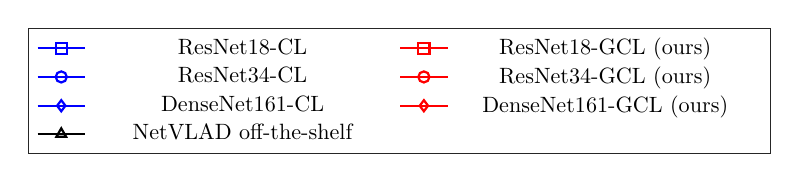
\begin{tikzpicture}[thick, scale=1, every node/.style={scale=.8}] 
    \begin{axis}[%
    hide axis,
    xmin=10,
    xmax=50,
    ymin=0,
    ymax=0.4, height=3.5cm, width=\columnwidth,
    legend style={draw=white!15!black,legend columns=2,legend style={minimum width=.41\columnwidth}},
    legend cell align={left}
    ]
    
\addlegendimage{blue, thick, mark size=2pt, mark=square};
\addlegendentry{ResNet18-CL};

\addlegendimage{red, thick, mark size=2pt, mark=square};
\addlegendentry{ResNet18-GCL (ours)};
\addlegendimage{blue, thick, mark size=2pt, mark=o};
\addlegendentry{ResNet34-CL};

\addlegendimage{red, thick, mark size=2pt, mark=o};
\addlegendentry{ResNet34-GCL (ours)};

\addlegendimage{blue, thick, mark size=2pt, mark=diamond};
\addlegendentry{DenseNet161-CL};

\addlegendimage{red, thick, mark size=2pt, mark=diamond};
\addlegendentry{DenseNet161-GCL (ours)};
\addlegendimage{black, thick, mark size=2pt, mark=triangle};
\addlegendentry{NetVLAD off-the-shelf};

\end{axis}
\end{tikzpicture}
\end{minipage}

    \end{subfigure}
  
    \setcounter{subfigure}{0}
\begin{subfigure}{\columnwidth}
\begin{tikzpicture}[thick, scale=1, every node/.style={scale=.75}]
\begin{axis}
[xlabel=K,
ylabel=Recall@K (\%), ylabel style={at={(axis description cs:0.05,0.5)}},grid, height=6cm, width=\columnwidth]
\addplot[black, thick, mark size=2pt, mark=triangle] table [x=k, y=r, col sep=comma] {plot_data/TB_Places/TB_Places_W18_W17_NetVLAD_recalls.csv};
%\addlegendentry{NetVLAD off-the-shelf};
%ResNet18
\addplot[red, thick, mark size=2pt, mark=square] table [x=k, y=r, col sep=comma] {plot_data/TB_Places/TB_Places_ResNet18_avg_2last_soft_siamese_w18_w17_recall_toplot.txt};
\addplot[blue, thick, mark size=2pt, mark=square] table [x=k, y=r, col sep=comma] {plot_data/TB_Places/TB_Places_ResNet18_avg_2last_binary_siamese_w18_w17_recall_toplot.txt};
%\addlegendentry{ResNet18-GCL};
%ResNet34

%\addlegendentry{ResNet34-GCL};
\addplot[red, thick, mark size=2pt, mark=o] table [x=k, y=r, col sep=comma] {plot_data/TB_Places/TB_Places_ResNet34_avg_2last_soft_siamese_w18_w17_recall_toplot.txt};
\addplot[blue, thick, mark size=2pt, mark=o] table [x=k, y=r, col sep=comma] {plot_data/TB_Places/TB_Places_ResNet34_avg_2last_binary_siamese_w18_w17_recall_toplot.txt};

\addplot[blue, thick, mark size=2pt, mark=diamond] table [x=k, y=r, col sep=comma] {plot_data/TB_Places/TB_Places_W18_W17_CAIP_recalls.csv};
%\addlegendentry{DenseNet161, BCL};
\addplot[red, thick, mark size=2pt, mark=diamond] table [x=k, y=r, col sep=comma] {plot_data/TB_Places/TB_Places_W18_W17_Soft_recalls.csv};
%\addlegendentry{DenseNet161-GCL (ours)};
\end{axis}
\end{tikzpicture}
\caption{Map: W17, Query: W18}
    \label{fig:w17_w18_recall}
\end{subfigure}
\begin{subfigure}{\columnwidth}
\begin{tikzpicture}[thick, scale=1, every node/.style={scale=.75}]
\begin{axis}
[xlabel=K,
ylabel=Recall@K (\%), ylabel style={at={(axis description cs:0.05,0.5)}},
legend pos =south east,grid, height=6cm, width=\columnwidth]
\addplot[black, thick, mark size=2pt, mark=triangle] table [x=k, y=r, col sep=comma] {plot_data/TB_Places/TB_Places_map_query_NetVLAD_recalls.csv};
%\addlegendentry{NetVLAD off-the-shelf};
\addplot[red, thick, mark size=2pt, mark=square] table [x=k, y=r, col sep=comma] {plot_data/TB_Places/TB_Places_ResNet18_avg_2last_soft_siamese_w18_map_query_recall_toplot.txt};
\addplot[blue, thick, mark size=2pt, mark=square] table [x=k, y=r, col sep=comma] {plot_data/TB_Places/TB_Places_ResNet18_avg_2last_binary_siamese_w18_map_query_recall_toplot.txt};
%\addlegendentry{ResNet18-GCL};

\addplot[red, thick, mark size=2pt, mark=o] table [x=k, y=r, col sep=comma] {plot_data/TB_Places/TB_Places_ResNet34_avg_2last_soft_siamese_w18_map_query_recall_toplot.txt};
\addplot[blue, thick, mark size=2pt, mark=o] table [x=k, y=r, col sep=comma] {plot_data/TB_Places/TB_Places_ResNet34_avg_2last_binary_siamese_w18_map_query_recall_toplot.txt};
%\addlegendentry{ResNet34-GCL};

\addplot[blue, thick, mark size=2pt, mark=diamond] table [x=k, y=r, col sep=comma] {plot_data/TB_Places/TB_Places_map_query_CAIP_recalls.csv};
%\addlegendentry{DenseNet161, BCL};
\addplot[red, thick, mark size=2pt, mark=diamond] table [x=k, y=r, col sep=comma] {plot_data/TB_Places/TB_Places_map_query_Soft_recalls.csv};
%\addlegendentry{DenseNet161-GCL (ours)};
\end{axis}
\end{tikzpicture}
\caption{Map: W18, Query: W18}
    \label{fig:w18_map_query_recall}
\end{subfigure}
   \caption{Results on the TB-Places dataset. In (a) the results when using W17 as map and W18 as query set. In (b) the top-k recall achieved when dividing W18 into map and query. }%The results achieved by our method are shown in red, the results of the models trained with the binary Contrastive Loss are in blue, and the results of NetVLAD are displayed in black.}
       \label{fig:tb_places_recall}
\end{figure}



\paragraph{Experiments and results}
We trained our method on the TB-Places dataset and show the results in Fig.~\ref{fig:tb_places_recall}. We considered three  backbones, namely ResNet18, ResNet34, and DenseNet161, which learn descriptors of size 512, 512 and 2208, respectively. We trained them with the binary Contrastive Loss function and with our Generalized Contrastive Loss function. Furthermore, we compare them with the NetVLAD off-the-shelf model. For these experiments we use only a Global Average Pooling.



\begin{figure*}[!t]
\begin{subfigure}{.24\columnwidth}
\begin{tikzpicture}[thick, scale=1, every node/.style={scale=.8}]
\begin{axis}
[xlabel=K,
ylabel=Recall@K (\%), ylabel style={at={(axis description cs:0.1,0.5)}},grid, height=4.75cm, width=\columnwidth,xtick distance=5, ytick distance=5]
\addplot[black, thick, mark size=2pt, mark=triangle] table [x=k, y=r, col sep=comma] {plot_data/7Scenes/PR_7scenes_recallatk_50FOV_heads_NetVLAD_recalls.csv};
\addplot[blue, thick, mark size=2pt, mark=o] table [x=k, y=r, col sep=comma] {plot_data/7Scenes/PR_7scenes_recallatk_50FOV_heads_ResNet18_crisp_recalls.csv};
\addplot[red, thick, mark size=2pt, mark=o] table [x=k, y=r, col sep=comma] {plot_data/7Scenes/PR_7scenes_recallatk_50FOV_heads_ResNet18_soft_recalls.csv};

\addplot[blue, thick, mark size=2pt, mark=square] table [x=k, y=r, col sep=comma] {plot_data/7Scenes/PR_7scenes_recallatk_50FOV_heads_ResNet34_crisp_recalls.csv};
\addplot[red, thick, mark size=2pt, mark=square] table [x=k, y=r, col sep=comma] {plot_data/7Scenes/PR_7scenes_recallatk_50FOV_heads_ResNet34_soft_recalls.csv};
\end{axis}
\end{tikzpicture}
    \caption{Heads}
    \label{fig:7Scenes_heads_recall}
\end{subfigure}~
\begin{subfigure}{.24\columnwidth}
\begin{tikzpicture}[thick, scale=1, every node/.style={scale=.8}]
\begin{axis}
[xlabel=K,
ylabel=Recall@K (\%), ylabel style={at={(axis description cs:0.1,0.5)}},grid, height=4.75cm, width=\columnwidth,xtick distance=5, ytick distance=5]
\addplot[black, thick, mark size=2pt, mark=triangle] table [x=k, y=r, col sep=comma] {plot_data/7Scenes/PR_7scenes_recallatk_50FOV_stairs_NetVLAD_recalls.csv};
\addplot[blue, thick, mark size=2pt, mark=o] table [x=k, y=r, col sep=comma] {plot_data/7Scenes/PR_7scenes_recallatk_50FOV_stairs_ResNet18_crisp_recalls.csv};
\addplot[red, thick, mark size=2pt, mark=o] table [x=k, y=r, col sep=comma] {plot_data/7Scenes/PR_7scenes_recallatk_50FOV_stairs_ResNet18_soft_recalls.csv};

\addplot[blue, thick, mark size=2pt, mark=square] table [x=k, y=r, col sep=comma] {plot_data/7Scenes/PR_7scenes_recallatk_50FOV_stairs_ResNet34_crisp_recalls.csv};
\addplot[red, thick, mark size=2pt, mark=square] table [x=k, y=r, col sep=comma] {plot_data/7Scenes/PR_7scenes_recallatk_50FOV_stairs_ResNet34_soft_recalls.csv};
\end{axis}
\end{tikzpicture}
    \caption{Stairs}
    \label{fig:7Scenes_stairs_recall}
\end{subfigure}~
\begin{subfigure}{.24\columnwidth}
\begin{tikzpicture}[thick, scale=1, every node/.style={scale=.8}]
\begin{axis}
[xlabel=K,
ylabel=Recall@K (\%), ylabel style={at={(axis description cs:0.1,0.5)}},grid, height=4.75cm, width=\columnwidth,xtick distance=5, ytick distance=5]
\addplot[black, thick, mark size=2pt, mark=triangle] table [x=k, y=r, col sep=comma] {plot_data/7Scenes/PR_7scenes_recallatk_50FOV_pumpkin_NetVLAD_recalls.csv};
\addplot[blue, thick, mark size=2pt, mark=o] table [x=k, y=r, col sep=comma] {plot_data/7Scenes/PR_7scenes_recallatk_50FOV_pumpkin_ResNet18_crisp_recalls.csv};
\addplot[red, thick, mark size=2pt, mark=o] table [x=k, y=r, col sep=comma] {plot_data/7Scenes/PR_7scenes_recallatk_50FOV_pumpkin_ResNet18_soft_recalls.csv};

\addplot[blue, thick, mark size=2pt, mark=square] table [x=k, y=r, col sep=comma] {plot_data/7Scenes/PR_7scenes_recallatk_50FOV_pumpkin_ResNet34_crisp_recalls.csv};
\addplot[red, thick, mark size=2pt, mark=square] table [x=k, y=r, col sep=comma] {plot_data/7Scenes/PR_7scenes_recallatk_50FOV_pumpkin_ResNet34_soft_recalls.csv};
\end{axis}
\end{tikzpicture}
    \caption{Pumpkin}
    \label{fig:7Scenes_pumpkin_recall}
\end{subfigure}~
\begin{subfigure}{.4\columnwidth}
\begin{minipage}[c][2cm]{\columnwidth}
\vspace{10pt}
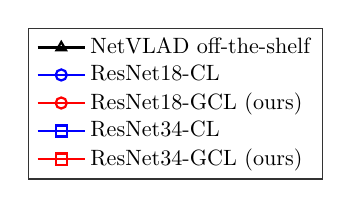
\begin{tikzpicture}[thick, scale=1, every node/.style={scale=.8}] 
    \begin{axis}[%
    hide axis,
    xmin=10,
    xmax=70,
    ymin=0,
    ymax=0.4,
    legend pos =north west,
    legend style={draw=white!20!black,legend cell align=left}, height=4.75cm, width=.61\columnwidth
    ]
    \addlegendimage{black, thick, mark size=2pt, mark=triangle}
    \addlegendentry{NetVLAD off-the-shelf};
    \addlegendimage{blue, thick, mark size=2pt, mark=o}
    \addlegendentry{ResNet18-CL};
    \addlegendimage{red, thick, mark size=2pt, mark=o}
    \addlegendentry{ResNet18-GCL (ours)};
    \addlegendimage{blue, thick, mark size=2pt, mark=square}
    \addlegendentry{ResNet34-CL};
    \addlegendimage{red, thick, mark size=2pt, mark=square}
    \addlegendentry{ResNet34-GCL (ours)};
    \end{axis}
    \end{tikzpicture} 
    \end{minipage}

\end{subfigure}

\setcounter{subfigure}{3}

\begin{subfigure}{.24\columnwidth}
\begin{tikzpicture}[thick, scale=1, every node/.style={scale=.8}]
\begin{axis}
[xlabel=K,
ylabel=Recall@K (\%), ylabel style={at={(axis description cs:0.1,0.5)}},grid, height=4.75cm, width=\columnwidth,xtick distance=5, ytick distance=5]
\addplot[black, thick, mark size=2pt, mark=triangle] table [x=k, y=r, col sep=comma] {plot_data/7Scenes/PR_7scenes_recallatk_50FOV_fire_NetVLAD_recalls.csv};
\addplot[blue, thick, mark size=2pt, mark=o] table [x=k, y=r, col sep=comma] {plot_data/7Scenes/PR_7scenes_recallatk_50FOV_fire_ResNet18_crisp_recalls.csv};
\addplot[red, thick, mark size=2pt, mark=o] table [x=k, y=r, col sep=comma] {plot_data/7Scenes/PR_7scenes_recallatk_50FOV_fire_ResNet18_soft_recalls.csv};

\addplot[blue, thick, mark size=2pt, mark=square] table [x=k, y=r, col sep=comma] {plot_data/7Scenes/PR_7scenes_recallatk_50FOV_fire_ResNet34_crisp_recalls.csv};
\addplot[red, thick, mark size=2pt, mark=square] table [x=k, y=r, col sep=comma] {plot_data/7Scenes/PR_7scenes_recallatk_50FOV_fire_ResNet34_soft_recalls.csv};
\end{axis}
\end{tikzpicture}
    \label{fig:7Scenes_fire_recall}
\caption{Fire}
\end{subfigure}~
\begin{subfigure}{.24\columnwidth}
\begin{tikzpicture}[thick, scale=1, every node/.style={scale=.8}]
\begin{axis}
[xlabel=K,
ylabel=Recall@K (\%), ylabel style={at={(axis description cs:0.1,0.5)}},grid, height=4.75cm, width=\columnwidth,xtick distance=5, ytick distance=5]
\addplot[black, thick, mark size=2pt, mark=triangle] table [x=k, y=r, col sep=comma] {plot_data/7Scenes/PR_7scenes_recallatk_50FOV_redkitchen_NetVLAD_recalls.csv};
\addplot[blue, thick, mark size=2pt, mark=o] table [x=k, y=r, col sep=comma] {plot_data/7Scenes/PR_7scenes_recallatk_50FOV_redkitchen_ResNet18_crisp_recalls.csv};
\addplot[red, thick, mark size=2pt, mark=o] table [x=k, y=r, col sep=comma] {plot_data/7Scenes/PR_7scenes_recallatk_50FOV_redkitchen_ResNet18_soft_recalls.csv};

\addplot[blue, thick, mark size=2pt, mark=square] table [x=k, y=r, col sep=comma] {plot_data/7Scenes/PR_7scenes_recallatk_50FOV_redkitchen_ResNet34_crisp_recalls.csv};
\addplot[red, thick, mark size=2pt, mark=square] table [x=k, y=r, col sep=comma] {plot_data/7Scenes/PR_7scenes_recallatk_50FOV_redkitchen_ResNet34_soft_recalls.csv};
\end{axis}
\end{tikzpicture}
    \caption{Redkitchen}
    \label{fig:7Scenes_redkitchen_recall}
\end{subfigure}~
\begin{subfigure}{.24\columnwidth}
\begin{tikzpicture}[thick, scale=1, every node/.style={scale=.8}]
\begin{axis}
[xlabel=K,
ylabel=Recall@K (\%), ylabel style={at={(axis description cs:0.1,0.5)}},grid, height=4.75cm, width=\columnwidth,xtick distance=5, ytick distance=5]
\addplot[black, thick, mark size=2pt, mark=triangle] table [x=k, y=r, col sep=comma] {plot_data/7Scenes/PR_7scenes_recallatk_50FOV_chess_NetVLAD_recalls.csv};
\addplot[blue, thick, mark size=2pt, mark=o] table [x=k, y=r, col sep=comma] {plot_data/7Scenes/PR_7scenes_recallatk_50FOV_chess_ResNet18_crisp_recalls.csv};
\addplot[red, thick, mark size=2pt, mark=o] table [x=k, y=r, col sep=comma] {plot_data/7Scenes/PR_7scenes_recallatk_50FOV_chess_ResNet18_soft_recalls.csv};

\addplot[blue, thick, mark size=2pt, mark=square] table [x=k, y=r, col sep=comma] {plot_data/7Scenes/PR_7scenes_recallatk_50FOV_chess_ResNet34_crisp_recalls.csv};
\addplot[red, thick, mark size=2pt, mark=square] table [x=k, y=r, col sep=comma] {plot_data/7Scenes/PR_7scenes_recallatk_50FOV_chess_ResNet34_soft_recalls.csv};
\end{axis}
\end{tikzpicture}
\caption{Chess}
    \label{fig:7Scenes_chess_recall}
\end{subfigure}~
\begin{subfigure}{.24\columnwidth}
\begin{tikzpicture}[thick, scale=1, every node/.style={scale=.8}]
\begin{axis}
[xlabel=K,
ylabel=Recall@K (\%), ylabel style={at={(axis description cs:0.1,0.5)}},grid, height=4.75cm, width=\columnwidth,xtick distance=5, ytick distance=5]
\addplot[black, thick, mark size=2pt, mark=triangle] table [x=k, y=r, col sep=comma] {plot_data/7Scenes/PR_7scenes_recallatk_50FOV_office_NetVLAD_recalls.csv};
\addplot[blue, thick, mark size=2pt, mark=o] table [x=k, y=r, col sep=comma] {plot_data/7Scenes/PR_7scenes_recallatk_50FOV_office_ResNet18_crisp_recalls.csv};
\addplot[red, thick, mark size=2pt, mark=o] table [x=k, y=r, col sep=comma] {plot_data/7Scenes/PR_7scenes_recallatk_50FOV_office_ResNet18_soft_recalls.csv};

\addplot[blue, thick, mark size=2pt, mark=square] table [x=k, y=r, col sep=comma] {plot_data/7Scenes/PR_7scenes_recallatk_50FOV_office_ResNet34_crisp_recalls.csv};
\addplot[red, thick, mark size=2pt, mark=square] table [x=k, y=r, col sep=comma] {plot_data/7Scenes/PR_7scenes_recallatk_50FOV_office_ResNet34_soft_recalls.csv};
\end{axis}
\end{tikzpicture}
    \caption{Office}
    \label{fig:7Scenes_office_recall}
\end{subfigure}
\caption{Recall@K results achieved on the 7 Scenes dataset. The results of the models trained with our Generalized Contrastive Loss are shown in red, while those of the models trained with the binary Contrastive Loss are shown in blue. The Recall@K achieved by NetVLAD off-the-shelf is plotted in black.}
\label{fig:recallat_k_7scenes}

\end{figure*}



We report results of two experiments. For the first one, we used the training set W17 as map, and the W18 set as query. With this experiment we tested the strength of the descriptors against significant variations between the query and the map set. We show the results in Fig.~\ref{fig:w17_w18_recall}. For the second experiment, we divided the W18 set into map and query, to test the generalization capabilities when both map and query sets are unknown to the place recognition model (i.e. not seen during training). The results are displayed in Fig.~\ref{fig:w18_map_query_recall}.
%
For both experiments the models trained with GCL and the proposed similarity ground truth consistently achieve better recall than the ones trained with the binary Contrastive Loss, with the exception of the ResNet18. %In some cases the models trained with the binary ground truth do not outperform the NetVLAD model, even though this one is not trained on the TB-Places dataset.




\section{Results on the 7Scenes dataset}

\paragraph{The dataset}
A benchmark dataset for indoor camera localization~\cite{Shotton2013}. It includes 26k training images and 17k test images, taken in seven environments. Each image has an associated ground truth 6DOF camera pose. Additionally, a 3D reconstruction of each scene is available. We use it to test our VPR models in indoor environments. For evaluation purposes, we define an image pair as a positive match if their annotated degree of similarity is higher than $50\%$. We use the training set as map, and the test set as query.


\paragraph{Experiments and results}
\label{sec:results7scenes}
We report the results in Fig.~\ref{fig:recallat_k_7scenes}. We used the ResNet18 and ResNet34 architectures as backbones with a Global Average Pooling layer and we compare them to NetVLAD off-the-shelf.  We achieved generally higher Recall@K results for the models trained using the GCL function, for all scenes. The cases of the \emph{stairs}  (Fig.~\ref{fig:7Scenes_stairs_recall}), \emph{chess}  (Fig.~\ref{fig:7Scenes_chess_recall}) and \emph{office} (Fig.~\ref{fig:7Scenes_office_recall}) scenes are particularly interesting, since with the GCL descriptors we are able to retrieve positive matches for nearly all the query images, with a top-5 recall for \mbox{ResNet34-GCL} of 98.1\%, 98.2\%  and 99.7\%, respectively.

Furthermore, we report the average precision results in Table~\ref{tab:ap-7scenes}. %This measure is an approximation of the area under the precision-recall curve and measures the number of pairs that can be correctly discriminated into positive and negative on the whole dataset. 
The models trained with the GCL function achieved higher AP than their corresponding models trained with the binary CL function. We achieved an average AP equal to 0.89 using the ResNet34-GCL model. %\revised{Following the general expectation that improved retrieval results would contribute to a better localization, we performed a small-scale localization experiment to compare the contribution of the GCL and CL training to the localization performance of an InLoc pipeline~\cite{taira2018inloc}. We report the results in the supplementary materials.}

%Finally, we tested the impact that a model trained with the GCL function and graded similarity has on the performance of a camera localization pipeline. We compared it to the case when the same model trained with the binary Contrastive Loss function is used for the image retrieval task, and report the localization error that we obtained in Table~\ref{tab:7scenes_loc}. For this experiment, we employed the InLoc algorithm~\cite{taira2018inloc}, using our learned representations with the ResNet34 backbone for the retrieval step. The images retrieved using the representation learned with GCL consistently led to an improvement of the localization accuracy w.r.t. the case in which the CL function is used. The enhanced performance of the retrieval task has a positive effect on the precision of localization algorithms.

%\subsection{\revised{Impact of na\"ive mining}} \revised{add and comment batch composition results}

\begin{table}[t!]
\centering
\caption{Average Precision results obtained by the networks trained with the proposed Generalized Contrastive loss function on the 7Scenes  dataset, compared with those achieved by the same network architectures trained using the binary Contrastive loss function and by the NetVLAD off-the-shelf model. }
\label{tab:ap-7scenes}

\renewcommand{\arraystretch}{1.0}
\resizebox{\textwidth}{!}{%
\begin{tabular}{@{\extracolsep{4pt}}lccccc@{}}
\toprule
\textbf{}   & \textbf{NetVLAD}       & \multicolumn{2}{c}{\textbf{ResNet18}} & \multicolumn{2}{c}{\textbf{ResNet34}} \\ 
\cmidrule{2-2}
\cmidrule{3-4}
\cmidrule{5-6}
\textbf{Scene}       & \textbf{off-the-shelf} & \textbf{CL}       & \textbf{GCL}               & \textbf{CL}       & \textbf{GCL}             \\ \midrule 
Heads      & 0.587        & 0.739   & 0.807           & 0.759   & \textbf{0.853}   \\
Stairs     & 0.533        & 0.855   & 0.883            & 0.884   & \textbf{0.944}   \\
Pumpkin    & 0.491        & 0.768   & 0.849            & 0.782   & \textbf{0.914}   \\
Fire       & 0.539        & 0.786   & \textbf{0.811}   & 0.796   & 0.803            \\
Redkitchen & 0.439        & 0.790   & 0.876            & 0.782   & \textbf{0.902}   \\
Chess      & 0.645        & 0.943   & 0.964 & 0.945   & \textbf{0.974}   \\
Office     & 0.399        & 0.794   & 0.890            & 0.802   & \textbf{0.896}   \\ \midrule
\textit{Mean }      & 0.519        & 0.811   & 0.868            & 0.821   & \textbf{0.898}   \\ \bottomrule
\end{tabular}}
\end{table}



\begin{figure*}[!t]
    \centering
    \includegraphics[width=0.9\textwidth]{figures/appendix/activations_transposed.pdf}
    %{\fontsize{8pt}{11pt}
    %\def\svgwidth{\textwidth}
    %  \input{figures/appendix/activations.pdf_tex}}
    \caption{CNN activations for the ResNet50-GeM and the VGG16-GeM models with CL and GCL for several input image pairs. The first two pairs, corresponding to the first four columns, are part of the MSLS test set. The third and fourth belong to the Pittsburgh30k and Tokyo 24/7 test set, respectively. We show the activations for the last layer of the backbone overlapped with the input images.}
    \label{fig:activations}
\end{figure*}


\section{GCL vs CL: Activation maps}
In Fig.~\ref{fig:activations}, we show the activation maps of the last convolutional layer of our models with a VGG16-GeM and a ResNet50-GeM backbone, both trained using the Contrastive Loss function (CL) and the proposed Generalized Contrastive Loss (GCL) function.  We selected two example image pairs from the MSLS test set~\cite{msls} (Kampala and Stockholm), one from the Pittsburgh30k test set~\cite{Arandjelovic2017}, and one from the Tokyo 24/7 dataset~\cite{Torii-CVPR2013}. For all cases, we observed that the model trained with the GCL function produces higher activation for the common visual features of the images, and lower for the irrelevant parts (i.e. the road or the sky), in contrast to the model trained with the binary CL, which focuses less in the concerned areas of the pictures. In the example from Stockholm we can observe that our model does not respond to the cars (which vary from picture to picture), while it does respond strongly to the cranes (which are a longer-term cue). The example from Tokyo 24/7 is also particularly interesting: our model trained with the GCL function has high responses on the common parts of the images even under big changes of illumination. We observed that ResNet architectures tend to produce a peak of activation on the top left corner of the images. This does not seem to occur with the VGG architecture, so our intuition is that this artifact is due to the residual computation. 






\section{Gradient of the Generalized Contrastive Loss}
Let us consider two input images $x_i$ and $x_j$, their latent representations $\hat{f}(x_i)$ and $\hat{f}(x_j)$, and define $ d(x_i, x_j)$ the Euclidean distance between the representations, such as:
\begin{equation}
\nonumber
 d(x_i, x_j) = \left \| \hat{f}(x_i)-\hat{f}(x_j) \right \|_2
\end{equation}
For simplicity of notation, hereinafter we refer to $d(x_i, x_j)$ as $d$.

\subsection{Contrastive loss}

\noindent The Contrastive Loss function is defined as:
\begin{equation}
\nonumber
\mathcal{L}_{CL}=\begin{cases}
\frac{1}{2} d ^2 ,& \text{if } y= 1\\
\frac{1}{2}\max(\tau- d ,0)^2,& \text{if } y=0
\end{cases}
\end{equation}
\noindent where $y$ corresponds to the binary ground truth label and $\tau$ corresponds to the margin.

\noindent In order to compute the gradient for this function, we consider three cases, depending on the ground truth label $y$ and the value of the distance $d$. 

\noindent \textbf{Case 1) $y=1$}

\noindent The loss function becomes:
\begin{equation}
    \nonumber
    \mathcal{L}_{CL}=\frac{1}{2} d ^2
\end{equation}

\noindent and its derivative with respect to $d$ is:
\begin{align}
\nonumber
\begin{split}
    \nabla  \mathcal{L}_{CL} = \frac{\partial}{\partial d} \left( \mathcal{L}_{CL} \right) =\frac{\partial}{\partial d} \left( \frac{1}{2} d^2 \right)=  d
\end{split}
\end{align}

\noindent \textbf{Case 2) $y=0, d < \tau$}
\noindent The loss function becomes:
\begin{equation}
    \nonumber
    \mathcal{L}_{CL}=\frac{1}{2}(\tau- d)^2
\end{equation}

\noindent and its derivative with respect to $d$ is:
\begin{align*}
\nonumber
\begin{split}
\nabla {} \mathcal{L}_{CL}=&
\frac{\partial}{\partial d} \left(  \mathcal{L}_{CL} \right) =\frac{\partial}{\partial d} \left[ \frac{1}{2}(\tau- d)^2 \right]=(\tau-d)(-1)= d-\tau
\end{split}
\end{align*}

\noindent  \textbf{Case 3) $y=0, d \geq \tau$}
\begin{equation}
    \nonumber
    \mathcal{L}_{CL} = 0
\end{equation}
and the gradient $\mathcal{L}_{CL} = 0$ as well. Thus, case 2 and case 3, for $y=0$, can be grouped as: 
%\textbf{Case 2 and Case 3 simplification, $y=0$}

\begin{equation}
    \nonumber
     \nabla  \mathcal{L}_{CL}=\begin{cases}
     d-\tau ,& \text{if } d < \tau\\
    0 ,& \text{if } d \geq \tau
\end{cases}
\end{equation}

\noindent and simplified as:

\begin{equation}
    \nonumber
     \nabla  \mathcal{L}_{CL}=\min( d-\tau,0)
\end{equation}

\noindent Finally, the \textbf{gradient of the Contrastive Loss function} is:

\begin{equation}
\nonumber
     \nabla  \mathcal{L}_{CL}=\begin{cases}
     d ,& \text{if } y= 1\\
    \min( d-\tau,0) ,& \text{if } y=0
\end{cases}
\end{equation}

%
\subsection{Generalized Contrastive loss}
We defined the Generalized Contrastive Loss function as:
\begin{equation}
\nonumber
 \mathcal{L}_{GCL}= \psi_{i,j}\cdot \frac{1}{2}d^2 + (1-\psi_{i,j}) \cdot \frac{1}{2}\max(\tau-d,0)^2
\end{equation}
\noindent where $\psi_{i,j}$ is the ground truth degree of similarity between the input images $x_i$ and $x_j$, and its values are in the interval $[0,1]$.
To compute the gradient of the GCL function we consider two cases, namely when 1) the distance $d$ between the representations is lower than the margin $\tau$ and 2) the alternative case when $d$ is larger than $\tau$. 

\noindent \textbf{Case 1) $d < \tau$}
\noindent The Generalized Contrastive loss function becomes:

\begin{equation}
\nonumber
 \mathcal{L}_{GCL}= \psi_{i,j}\cdot \frac{1}{2}d^2 + (1-\psi_{i,j}) \cdot \frac{1}{2}(\tau-d)^2 
\end{equation}

\noindent and its derivative with respect to $d$ is:
\begin{align*} 
\nonumber
\begin{split}
\nabla  \mathcal{L}_{GCL}=\frac{\partial}{\partial d} \left[ \psi_{i,j} \cdot \frac{1}{2} d^2  + (1 - \psi_{i,j}) \cdot \frac{1}{2}(\tau - d)^2 \right]=\\
=\psi_{i,j} \cdot d + (1-\psi_{i,j}) (\tau-d)(-1)=
% \\&=\psi_{i,j} \cdot d + (1 - \psi_{i,j}) \cdot (d - \tau)=
\\=\psi_{i,j} \cdot d + d - \tau- \psi_{i,j} \cdot d + \psi_{i,j} \cdot \tau =
%\\&=d-\tau+\psi_{i,j}\cdot\tau=
%\\&=d+\tau(-1+\psi_{i,j})=
\\=d+\tau(\psi_{i,j} -1)
\end{split}
\end{align*}

\noindent \textbf{Case 2) $d \geq \tau$}

\noindent The Generalized Contrastive loss function becomes:
\begin{equation}
\nonumber
 \mathcal{L}_{GCL}= \psi_{i,j}\cdot \frac{1}{2}d^2 + (1-\psi_{i,j}) \cdot \frac{1}{2}(0)^2 = \psi_{i,j}\cdot \frac{1}{2}d^2
\end{equation}

\noindent and its derivative with respect to $d$ is:
\begin{equation}
    \nonumber
\nabla \mathcal{L}_{GCL}=
\frac{\partial}{\partial d}\mathcal{L}_{GCL}=
\frac{\partial}{\partial d} \left[ \psi_{i,j}\cdot \frac{1}{2} d^2  \right] = 
d \cdot \psi_{i,j}
\end{equation} 


\noindent Finally, the \textbf{gradient of the Generalized Contrastive Loss function} is:
\begin{equation}
     \nabla  \mathcal{L}_{GCL}=\begin{cases}d+\tau(\psi_{i,j}-1),& \text{if } d<\tau\\
     d \cdot \psi_{i,j},& \text{if } d \geq \tau\\
     \end{cases}
\end{equation} 





